\documentclass[12pt]{report}

\usepackage[utf8]{inputenc}
\usepackage{amsmath}
\usepackage{amsfonts}
\usepackage{amssymb}

% Line spacing
\usepackage{setspace}
%\onehalfspacing
\doublespacing

% Figures
\usepackage{caption}
\usepackage{graphicx}
\usepackage{hyperref}
\usepackage{multirow}

% Matrix packages
\usepackage{blkarray}
\usepackage{amsmath}

% Code blocks
\usepackage{fancyvrb}
\usepackage{tcolorbox}

% Margin adustment
\usepackage[margin=1in]{geometry}
%\addtolength{\oddsidemargin}{-1in}
%\addtolength{\evensidemargin}{-1in}
%\addtolength{\textwidth}{1.75in}
%\addtolength{\topmargin}{-1in}
%\addtolength{\textheight}{1.75in}

% Paragraph indentation
\usepackage{changepage}

\author{Lillian Tatka}
\title{In Silico Evolution of Oscillating Mass-Action Chemical Reaction Networks}
\begin{document}
\begin{titlepage}
\begin{center}

%\begin{spacing}{1.5}
%Internship Project Report\\
%\vspace*{\fill}
%\end{spacing}
\begin{spacing}{2.5}
In Silico Evolution of Oscillating Mass-Action Chemical Reaction Networks
\vspace*{\fill}
%\textit{Submitted by}
\end{spacing}

\begin{spacing}{1.15}
Lillian Tatka

\vspace*{\fill}


A dissertation\\submitted in partial fulfillment of the\\requirements for the degree of
\\
\vspace*{\fill}
Doctor of Philosophy\\
\vspace*{\fill}
University of Washington\\
2024
\vspace{\fill}

Reading Committee:\\
Herbert Sauro, Chair\\
Patrick Boyle\\
Lucian Smith\\


\vspace*{\fill}
Program Authorized to Offer Degree:\\
Bioengineering

\end{spacing}
\end{center}
\end{titlepage}


\null
\begin{center}
\textcopyright Copyright 2024\\
Lillian Tatka
\end{center}
\pagenumbering{gobble}
\newpage

\pagenumbering{roman}
\begin{center}
University of Washington\\
\vspace*{\fill}
\textbf{Abstract} \\
\vspace*{\fill}
In Silico Evolution of Oscillating Mass-Action Chemical Reaction Networks\\
\vspace*{\fill}
Lillian Tatka\\
\vspace*{\fill}
Chair of the Supervisory Committee:\\
Herbert Sauro\\
Bioengineering
\pagenumbering{gobble}
\end{center}
\vspace*{\fill}
Computational models are increasingly used in high-impact decision making in science, engineering, and medicine. It is crucial that computational models meet a standard of credibility when using them in high-stakes decision making. For this reason, institutes including NASA, the FDA, and the EMA have developed standards to promote and assess the credibility of computational models and simulations. However, due to the breadth of models these institutes assess, these credibility standards are mostly qualitative and avoid making specific recommendations. On the other hand, modeling and simulation in systems biology is a narrower domain and several standards are already in place. These factors facilitate the development of a quantitative credibility standard. A systems biology credibility standard is essential given the rise in complexity and influence of models. This proposal describes the development of a testing suite to standardize and automate credibility testing and scoring of computational systems biology models. The test suite will include dynamic tests that examine the output of a simulated model, verification and validation tests, and a preliminary assessment of parameter sensitivity to gauge uncertainty in the model's predictions. 

\tableofcontents

\listoffigures

\listoftables

\chapter{Introduction}
\pagenumbering{arabic}
The \textit{in silico} evolution of chemical reaction networks can be a useful tool to create functional networks with specific behaviors as well as to investigate possible pathways of natural evolution. Large sets of synthetic networks can be useful for exploring design patterns and network motifs, gathering statistics network characteristics, benchmarking software, and informing design of synthetic networks. Although several studies use \textit{in silico} evolution to generate networks, the vast majority of them focus on genetic regulatory networks, and almost none of them provide software for others to reproduce their results or use evolutionary strategies in other work. A fast and user-friendly software package would allow researchers to experiment with \textit{in silico} evolution without significant knowledge of programming. 

The key objective of this work is to produce a software package that enables the \textit{in silico} evolution of mass-action chemical reaction networks and to explore features and hyperparameters of the evolutionary algorithm that influence the evolution of oscillatory reaction network. The software should be accessible to researchers with minimal programming experience, produce results relatively quickly, and be problem agnostic, meaning that a variety of behaviors could be evolved.  

This project began with the creation of a python tool to evolve oscillating chemical reaction networks. Described in chapter \ref{chap: cesium_paper}, this work was intended as a small initial step towards understanding the function of biochemical oscillators and identifying common design patterns that enable oscillation. Oscillating systems of are of particular interest due to their biological relevance and interesting dynamics and serve as a good candidate problem due to the presence of an intermediate state (damped oscillations). A large population of oscillators was computationally evolved and their reaction characteristics compared to non-oscillating systems. The library of reaction networks generated in this research was used to construct a publicly available database to enable further oscillator/design pattern research as well as to serve as a standardized data set for testing novel software and algorithms. 

However, the algorithm used to generate these oscillating networks had its flaws. It took a long time to execute, several minutes per run, and failed to generate oscillators most of the time. Only approximately 5\% of evolution trials would result in an oscillator. It took several days of computing time to generate the small database. The most likely cause of this low success rate was the rapid convergence of solutions. The design of the algorithm allowed the most fit reaction networks to dominate the population, even if they were not oscillators or close to becoming oscillators. This dominance would reduce the space for innovation and prevent more fit networks from developing. If a promising candidate network failed to develop in the first few generations, it was unlikely that the evolution trial would be successful.

Additionally, the structure of the code and algorithm did not allow for easy modification and exploration. For example, a user might wish to implement a different selection technique in an attempt to avoid the problem of rapid convergence, but the software was not created to allow for such tinkering. Users could modify some hyperparameters, such as the number of generations and population size, but the fundamental evolution algorithm could not be modified. 

To address these shortcomings and explore evolution strategies for mass-action reaction networks, a new software tool was developed, NetEvolve, described in detail in chapter \ref{chap: NetEvolve}. The software is written in the Julia programming language [CITTEEEEE], which uses just-in-time (JIT) compiling, type stability, and multiple dispatch to gain significant speed advantages over interpreted languages such as Python. The evolution algorithm can be used immediately using default settings or customized using a JSON file. By default, the algorithm evolves oscillators, but users could provide any time series data and the algorithm would attempt to generate networks to match. 

To combat premature convergence, NetEvolve separates candidate reaction networks into groups based on similarity. These groups are analogous to species in natural evolution and individuals are compared only against members of the same species. This prevents more fit candidate networks from dominating the population and shelters network innovations that may reduce fitness at first but develop into useful features over the course of several generations. 

Inspired by the use of evolutionary algorithms to create artificial neural networks, NetEvolve also implements a form of crossover, a mutation operator that combines features from two ``parent" networks to create a new ``offspring" network. This feature was shown to improve evolution performance when evolving artificial neural networks and genetic regulatory networks, but has been thought to be disruptive for evolving mass-action networks. The application of crossover to mass-action networks is explored in detail in chapter \ref{chap: NetEvolve}.

\begin{itemize}
\item\textbf{Aim 1:} Develop a python package to perform dynamic tests on systems biology models in order to assess their credibility
\item\textbf{Aim 2:} Create tools to automatically verify and validate models
\item\textbf{Aim 3:} Build software to automate simple parameter sensitivity analyses
\end{itemize}

This research will result in two first author publications, the titles of which are to be determined. The first publication will describe the design and purpose of the software package and include some preliminary examples of implementation. The second publication will present the full software package and demonstrate its use on several existing models. I hope to finish this work by June 2024.

\chapter{Background}

This chapter provides context for the major themes of this dissertation: chemical oscillators and evolutionary algorithms. This chapter begins with a brief introduction to computational chemical reaction network modeling. Section \ref{section:intro_oscillators} describes the motivations for focusing on oscillatory systems. Lastly, sections \ref{section:intro_GA}, \ref{section:tools_GA}, and \ref{section:tools_networks} describe the current state of evolutionary algorithms in systems biology, including relevant software tools.


\section{Introduction to Chemical Reaction Network Modeling}
\label{section:intro_crn}
The projects described here focus on computational models of (bio)chemical reaction networks (CRNs). Although several modeling paradigms exist to describe CRNs, this work uses CRNs represented by systems of ordinary differential equations. A CRN is a set of chemical reactions $R_i$ where i is the index over the range 1 to n, the total number of reactions in the network . Reactions involve the chemical species of the network, $S_j$ where j is the index of each species from 1 to the total number of species. A reaction is then represented as follows:
\begin{equation*}
Ri: \sum_{j\in S}^{}\alpha_{ij}S_j\to \sum_{j\in S}^{}\beta_{ij}S_j
\end{equation*}
where $\alpha_{ij}$ and $\beta_{ij}$ are non-negative integers, stoichiometry coefficients. For example, a simple 3-species, 2-reaction network can be represented by the following reactions:
\begin{equation}
\begin{split}
S1 + S2 \to S3 \\
S3 \to S1 + S2
\end{split}
\end{equation}
However, these reactions alone are insufficient to completely describe the small network.  Assuming mass-action kinetics, the rate at which a reaction proceeds is proportional to the concentration of the reactants. The constant of proportionality is referred to as the rate constant. To discern the dynamics of the system, the rate constants must be specified.

\begin{equation}
\begin{split}
S1 + S2 \to S3; \;\;\;\;\;\; k_1*S1*S2\\
S3 \to S1 + S2; \;\;\;\;\;\;\;\;\;\;\;\;\; k_2*S3
\end{split}
\end{equation}
The rate of change of each species can then be put in the form of a system of differential equations. When the initial concentrations of the species are given, this system can be solved numerically to describe the change of species concentrations over time.
\begin{equation}
\begin{split}
\frac{dS1}{dt}=k_2S3 - k_1S1S2\\
\frac{dS2}{dt}=k_2S3 -k_1S1S2\\
\frac{dS3}{dt}=k1S1S2 - k_2S3
\end{split}
\end{equation}

Chemical reaction network modeling is used across a variety of fields including pharmacology, biological sciences, physical chemistry, chemical engineering, and synthetic biology \textbf{CITATIONS}. To this end, numerous tools have been developed to aid in model development, description, and simulation. This dissertation introduces an additional software tool for exploring small chemical reaction networks. Of particular interest are chemical oscillators.


\section{Chemical Oscillators}
\label{section:intro_oscillators}

Chemical oscillators provide a tangible and accessible means to study the dynamics of nonlinear systems. They offer insights into how simple chemical reactions can produce complex, time-varying behaviors, shedding light on fundamental principles of dynamical systems theory. Understanding how these patterns emerge from the collective behavior of individual molecules can inform our understanding of the mechanisms underlying biological oscillations, providing insights into the molecular processes driving rhythmic behaviors in living organisms. This dissertation explores evolutionary algorithms in systems biology with focus on the generation and study of synthetic oscillatory networks.

\subsection{A Brief History}
The first oscillating chemical system was described in 1828. Gustav Fechner described and electrochemical cell that produced an oscillating current. Later, in 1899, Fredriech Ostwald observed that the rate of chromium dissolution in acid periodically increased and decreased. Both these systems were heterogenous mixtures, leading to the belief that homogenous oscillating reactions were impossible, a belief that persisted through much of the 20th century. Their relatively recent discovery and study makes homogenous chemical oscillators a topic of particular interest. 

In 1910, prior to leaving science to work for an insurance company, Alfred Lotka authored a monograph on theoretical biology \cite{Lotka1910}. He showed that a set of consecutive mass-action reactions can create damped oscillators which eventually settle at an equilibrium. A decade later he published a second paper on theoretical mass-action oscillatory systems \cite{Lotka1920, Lotka1920b}.

Shortly thereafter, physicist Vito Volterra's interest in mathematical biology was piqued by the observation that piscivorous fish had prospered in abandoned fisheries while populations of herbivrous fish remained constant. In 1926, he published a study to explain this phenomena proposing the same equations as Lotka, which he graciously acknowledged when Lotka penned a letter to Nature pointing out his publication of the same equations in 1925 \cite{Volterra, lotka-volterra}. The Lotka-Volterra model is well-known today as a simple representation of predator-prey interactions, where both populations oscillate in time. 

The Lotka-Volterra model consists of three irreversible steps describing the relationships between grass, rabbits, and lynxes. A represents grass, which is assumed to be constant. Rabbits, represented by X, consume grass to grow their population (equation \ref{eqn: LV_1}). Lynx, in turn, consume rabbits to grow their population (equation \ref{eqn: LV_2}) before eventually dying (equation \ref{eqn: LV_3}).

\begin{equation}
\label{eqn: LV_1}
A + X \to 2X
\end{equation}
\begin{equation}
\label{eqn: LV_2}
X + Y \to 2Y
\end{equation}
\begin{equation}
\label{eqn: LV_3}
Y \to P
\end{equation}

These ``reactions" assume ``mass-action" kinetics where the rate of each depends on the amount of grass (constant) and sizes of the population of rabbits and lynx respectively. These rates can be described by the following differential equations, where ${k_{y}}$ describes the rate of lynx reproduction given a rabbit of population size ${x}$, ${k_{d}}$ describes the mortality rate of lynx, and ${k_{x}}$ describes the rate at which rabbits reproduce. 

\begin{equation}
dx/dt = k_{x}ax - k_{y}xy
\end{equation}
\begin{equation}
dy/dt = k_{y}xy - k_{d}y
\end{equation}

The oscillations in this system result from the time delay between the growth in rabbit population growth and lynx population growth as well as the delay from rabbit population decline to lynx decline. Rabbits reproduce because grass is in constant supply. As the rabbit population grows, the lynx population follows as prey becomes plentiful. Once the lynx population gets too high, it will begin consuming rabbits at a rate faster than they can reproduce due to the constant supply of grass. Once the rabbit population declines, the lynx population will follow as food grows scarce and they begin to starve. When the lynx population is depleted, there will be less predation pressure and the population of rabbits will begin to grow again. This phenomenon can be observed in nature, as was carefully documented by Charles Elton in 1942 \cite{Elton1942}. The predator-prey model has also been demonstrated in the laboratory with paramecia that consume yeast \cite{Gause}.


\subsection{Dynamics}
A key feature of the Lotka-Volterra model, and of most chemical oscillating systems is the presence of autocatalysis. The rate of growth of a population increases as the size of the population increases. In chemical systems, Reactions are considered autocatalytic when the products increase the rate of reaction or when a chemical decelerates the rate of its own destruction~\cite{Tyson2004}
The prominence of autocatalysis is also observed in the evolution of \textit{in silico} theoretical chemical reaction networks, as is described in chapter \ref{chap: cesium_paper} \cite{Tatka2023}. 

Long lasting oscillations occur only if the proper feedback mechanism is present \cite{Sharma2006}. Often the feedback mechanism takes the form of autocatalysis. However, when unchecked, a system with autocatalysis can lead to explosion as the product concentration continues to build and increase the rate of product formation. An inhibition step is necessary to prevent this explosion of products. However, if autocatalysis and inhibition occur simultaneously, the steady state is stabilized and oscillation does not occur. The inhibition step must be delayed. Often this is accomplished by intermediate reactions. 

Oscillation can also be achieved with negative feedback \cite{Tyson1975, Sauro_dynamics}. In chemical reaction networks, this takes the form of end-product inhibition, where the final product in a series of reactions inhibits an enzyme from an earlier step in the sequence. A classic example of this is the repressilator, a three gene (or species) loop where each gene expresses a protein that represses the next gene in the loop (figure \ref{fig:repressilator}) \cite{Elowitz2000}. The invention of the repressilator was a landmark achievement in the field of synthetic biology showcasing the feasibility of engineering complex gene circuits with predefined functions. It provided a foundational framework for the design and construction of synthetic genetic oscillators and inspired subsequent research in the development of artificial gene regulatory networks.

\begin{figure}
    \centering
    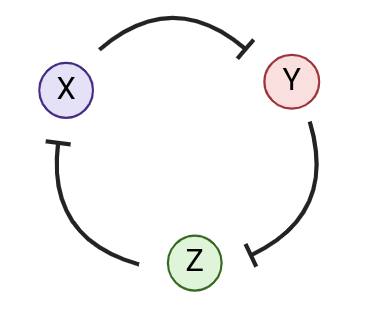
\includegraphics[width=7cm]{images/repressilator.png}
    \caption[Three node repressilator]{A three species repressilator.}
    \label{fig:repressilator}
\end{figure}

\subsection{Biological Relevance}
Oscillators are biological relevant beyond ecological interactions. A fundamental aspect of living systems, oscillators occur across several levels of biological organization. 

The circadian clock exemplifies a well-studied molecular oscillator that regulates daily rhythms in behavior, metabolism, and physiology across organisms \cite{circadianReview, circadianOverview}. At its core, the circadian clock consists of interconnected transcriptional-translational feedback loops involving clock genes and proteins. These feedback loops take the form of interconnected repressilators \cite{YAMASHINO2013, Pett2016}. These molecular oscillators synchronize cellular processes with the day-night cycle, optimizing organismal fitness and survival. Disruptions to circadian rhythms have profound implications for health, contributing to various disorders such as sleep disorders, metabolic syndrome, and mood disorders \cite{circadianReview}.


Beyond the circadian clock, molecular oscillators operate within cells to regulate diverse processes such as gene expression, signal transduction, and metabolic pathways. Examples include calcium oscillations \cite{Smedler2014}, cyclic AMP (cAMP) signaling \cite{Dyachok2006}, and oscillatory patterns of gene expression driven by transcriptional regulatory networks \cite{Cerone2012}. These intracellular oscillatory systems enable cells to respond dynamically to external stimuli, coordinate complex physiological responses, and maintain cellular homeostasis under changing conditions \cite{Cheong2010, Jolma2010}. Oscillations are also present in systems such as neuronal networks \cite{Cebolla2019}, cardiac muscle cells \cite{Weiss2010, Montano2001}, pancreatic beta cells \cite{Watts2014}, and glycolysis \cite{Ghosh1964}, among others, highlighting the importance of molecular oscillators in physiological function.

Synthetic oscillatory systems offer considerable potential for advancing biomedicine and biotechnology. These dynamic systems can serve as biosensors, detecting the presence and concentration of proteins, drugs, and other chemicals \cite{Kis2015, CubillosRuiz2021}. Synthetic genetic oscillators can be employed to modulate the local delivery of effector molecules to tumors \cite{CubillosRuiz2021}. More broadly, synthetic oscillators could serve as essential components for engineering complex synthetic gene and protein networks. These networks could be used for disease diagnosis, pharmaceutical screening, and bio-manufacturing or used therapeutically to modulate endogenous oscillating systems \cite{Kis2015}.




\section{Applications of Evolutionary and Genetic Algorithms in Systems Biology}
\label{section:intro_GA}
Genetic and evolutionary algorithms are optimization techniques inspired by the principles of natural selection and genetics. These algorithms mimic the process of natural evolution to solve complex optimization problems across various domains. At the core of genetic algorithms lies the concept of natural selection, a fundamental mechanism driving evolution in biological systems. Natural selection operates on populations of individuals, favoring those with traits that confer a reproductive advantage. Over successive generations, beneficial traits become more prevalent in the population, leading to the emergence of better-adapted individuals.






Evolutionary algorithms offer a computational framework for addressing the inherent complexity and nonlinearity of biological systems, providing a means to explore large solution spaces and optimize model parameters and structures.



The use of evolutionary algorithms in systems biology became popular in the late 1990s, often to better understand metabolic pathways. This approach has been used to demonstrate the optimality of the glycolysis \cite{Heinrich1999, stephani1999} and the Krebs citric acid cycle \cite{mittenthal2000}. In these studies, genetic algorithms were used to optimize reaction rates but not the structure of the networks.

Francois and Hakim evolved both the structure and reaction rates of genetic regulatory networks in an effort to generate small genetic networks that functioned as bistable switches and oscillators \cite{francois_hakim_2004}. The  algorithm used only mutation and selection, avoiding crossover, to minimize the difference between the candidate networks' output and idealized time series data displaying the desired behavior. Francois and Hakim argued that one of their evolved oscillators was structurally similar to the networks responsible for the circadian rhythm. However, Chu extended this work and found no consistent patterns in the evolved oscillators \cite{Chu_oscillator}. She noted that it is computationally unfeasible to thoroughly examine all resulting networks, but argued that the similarity to the circadian rhythm was likely coincidental. Despite Chu's study occurring almost 20 years ago, the problem of thoroughly pattern mining evolved networks remains and issue. The results of these works encouraged the exploration of evolutionary techniques on similar problems.

Fujimoto et al. employed a similar strategy to study genetic networks leading to striped patterning and ultimately body segmentation in arthropods \cite{fujimoto_network_2008}. When analyzing the resulting networks, they found three distinct classes, feed-forward loops, feed-back loops, and interconnections between the two. These three classes reproduced various segmentation strategies observed in arthropods.

Kobayashi et al. also explored the evolution of oscillatory genetic networks, however their algorithm fixed parameter values and only allowed connection rewiring to achieve oscillations with prescribed time periods \cite{kobayashi_evolutionary_2010}. Deckard and Sauro expanded this concept beyond genetic regulatory networks to evolve small networks with specific computational capabilities such as square root and cube route calculators \cite{deckard_preliminary_2004}. As with the previously mentioned algorithms, their algorithm avoided crossover relying solely on mutation to develop candidate solutions. Attempts to use crossover did not result in fitter offspring, possibly due to combining heterologous networks and thus disrupting developing solutions. This work was continued by Paladugu et al seeking to generate mass-action network functional modules with specific behaviors, including oscillators \cite{Paladugu2006}.  This algorithm avoided crossover as the authors argued that it would be disruptive.

Marchisio and Stelling argued that brute force optimization algorithms lack efficiency and that implementing some element of rational design could speed up automatic design of genetic networks implementing boolean logic gates \cite{marchisio_automatic_2011}. They separate structural and parameter optimization by first generating several possible circuits and then ranks feasibility based on the structure. Then the best solutions undergo parameter optimization. Separating structural design from parameter optimization certainly saves computation time, but it relies on the existence of a rational solution, and is better suited for genetic networks, where these attributes are more easily separated. For more complex tasks, a solution might depend on a precise combination of both structure and parameter.

Other approaches fix structure and make use of evolutionary algorithms to explore the parameter space while fixing network topology. Jin and Sendhoff used an evolution strategy to explore parameters of regulatory motifs with fixed structures \cite{jin_evolving_2008}. Porubsky and Sauro use an evolutionary algorithm to search for parameters that yield oscillations in mass-action networks of fixed structure \cite{porubsky2019}.

Most applications of evoltuionary algorithms in systems biology avoid the use of crossover as it tends to disrupt candidate solutions. For example, Drennan and Beer successfully evolved a repressilator (a specific type of oscillatory reaction netowrk \cite{Elowitz2000}) using a genetic algorithm that included crossover \cite{drennan_beer}. Instead of evolving sets of differential equations, Drennan and Beer encoded their genetic regulatory networks using strings of 4 different letters, analogous to DNA encoding. Knabe et al. used a similar approach to evolve oscillators that interact with the environment \cite{knabe}. This approach allows for the straightforward implementation of crossover, but limits the space of possible models. Due to this encoding, there was a high probability of breaking connections making it difficult to pass on structural innovations.

Stanley and Miikkulainen addressed this problem in 2002 with NEAT (NeuroEvolution of Augmenting Topologies), a powerful algorithm used for evolving artificial neural networks (ANNs) \cite{stanley_evolving_2002}. Unlike traditional methods of neural network training, which typically involve adjusting the weights and biases of fixed network architectures, NEAT evolves both the structure and weights of neural networks simultaneously. A two key features of NEAT are the use of a more meaningful structural crossover technique, and speciation, which protects innovations and allows them time to develop by having candidate solutions compete only against similar individuals instead of the entire population. Dinh et al. adapted this technique to genetic regulatory networks and found improved performance in evolving oscillators with the use of crossover.

\textbf{paragraph about how these are really just ways to change parameters}

\section{Tools for Evolutionary and Genetic Algorithms}
\label{section:tools_GA}
Although there are many tools that enable evolutionary algorithms and simulating chemical reaction networks, there are none that facilitate evolutionary algorithms using chemical reaction networks. The two main issues with packages described here are user-friendliness and network encoding.

All of the tools described here require at least basic programming knowledge. Some packages boast extreme customizability, but require the user to essentially use the package as building blocks to write their own evolutionary algorithm program. These tools have significant barriers for users who's focus is not software development and programming.

Perhaps the larger issue is that all packages described here are intended for ``classic" evolutionary algorithm applications, where solutions can be encoded as vectors or matrices of integers and floating point numbers. This is not the case for the problem of evolving reaction networks, where candidate solutions are entire networks. To completely describe a chemical reaction network, an encoding must include (at the minimum) numerous reactions, including reactants, products, and rate constants and initial concentrations for each chemical species.  

\subsection{Python Libraries}

Most packages for implementing genetic and evolutionary algorithms are written in python \cite{python3}. Python is one of the most ubiquitous programming languages frequently topping lists of the most commonly used languages. It is often used in scientific applications due to it being open source, easy to use, and having vast library support. Likely for these reasons, most existing evolutionary algorithm tools are python libraries.

Although likely not an exhaustive list, the main python packages for evolutionary and genetic algorithms are described here.


\subsubsection{DEAP}
In 2012, Fortin et al. released the python package DEAP (Distributed Evolutionary Algorithms in Python) \cite{DEAP_JMLR2012}. The packages offers a toolbox of evolutionary algorithm features including different types of crossover, evolutionary strategies, and mutation operators. Unlike other frameworks DEAP makes algorithm explicit and data structures transparent, as opposed to black-box frameworks. Although DEAP allows for extensive customization, individuals are represented as arrays of values. Users can customize these arrays, such as specifying integers or floats at specific locations, but individuals must be in this form. For most optimization problems, this representation is adequate, however it is difficult to fully represent a chemical reaction network in this form. Reaction networks have varying numbers of reaction, so a stoichiometry matrix would be inadequate unless it contained a row for every possible reaction. Additionally, reactions require rate constants, and networks require initial values for each species. 

But beyond the encoding issue, the DEAP package, while highly versatile and proven in many research application, requires extensive programming knowledge. For example to build a population, a user must: (1) register the data type for each gene, (2) register an individuals that combines these gene data types, (3) register a population that uses the individual, and finally (4) build the population. Running an entire genetic algorithm requires far more additional programming. 

\subsubsection{Pyevolve}
Pyevolve is more simple framework for genetic algorithms compared to DEAP but has limited features \cite{pyevolve}. Despite its relative simplicity, it still requires extensive programming knowledge to implement an evolutionary process and problems are still limited to those whose ``genes" can be encoded as arrays of numbers. 

Pyevolve also requires significantly more programming to accomplish the same task comapred to DEAP. DEAP requires 59 lines of code to solve the OneMax problem\footnote{The OneMax problem is a classic problem in the field of evolutionary computation. It is a simple bit sting problem where the objective is the maximize the number of ones in a binary string. The fitness of each individual is the total number of ones in its string. The simplicity of the OneMax problem makes it an ideal benchmark for testing optimization algorithms}, compared to 378 for pyevolve \cite{LEAP}. 

The most recent release was 2014 and the library is no longer maintained.

\subsubsection{EasyGA}
EasyGA is a more recent (2021) python tool for genetic algorithms \cite{easyGA}. EasyGA makes it relatively easy to implement simple genetic algorithms, but still requires the user to have some advanced programming knowledge. The simplicity of easyGA makes it useful to only selected problems due to gene encoding restrictions.

The library has a limited number of genetic operators. Additionally, EasyGA randomly mutates both parents and offspring, a feature that goes against the basic premise of genetic algorithms. 

At the time of writing, the EasyGA GitHub repository only had 47 stars, suggesting that it is infrequently used.

\subsubsection{LEAP}
LEAP (Library for Evolutionary Algorithms in Python) is another recently developed library published in 2020 \cite{LEAP}. LEAP was designed to simplify the process of implementing evolutionary and genetic algorithms. However, LEAP has some core design weaknesses that impact usability. 

Despite one of the objectives of LEAP being to simplify the process of implementing genetic algorithms, it still requires the user to write the evolution loop resulting in more code to solve simple problems. The user also has to manually increment the generation counter by calling a function specific to this purpose. Failing to call the function results in an infinite evolution loop, a problem that may not be immediately identifiable and solvable by less experienced users.

Additionally, LEAP has no means of tracing the results of each generation of evolution. This makes troubleshooting more difficult and renders LEAP an ineffective tool for those who may wish to study the evolution process and not just the final results.

LEAP is also a relatively unpopular choice for implementing evolutionary algorithms with only 77 stars at the time of writing.

\subsubsection{PyGAD}
In 2020, pyGAD was released with the aim to simplify the implementation of genetic algorithms for users with less programming experience while simultaneously proving control over ``everything possible" \cite{gad2023pygad}. PyGAD requires 3 core steps: (1) build the fitness function, (2) instantiate the relevant genetic algorithm class, (3) call the run function. The operation of pyGAD is relatively simple. Some programming knowledge is required for the user to create a fitness function and implement any further customization, but the bulk of the algorithm is run automatically. 

As with the other software tools described here, the main drawback of pyGAD for applications in systems biology is the restrictions on encoding individual solutions. Solutions must be encoded as a 1D vector of numbers. This is insufficient for evolving chemical reaction networks, where a solution is an entire reaction network and all parameters needed to simulate the network.

\subsubsection{EvoX}
Most recently, Huange et al. released EvoX, a python library for evolutionary computing \cite{Huang2024}. Unlike other libraries described here, EvoX is optimized for distributed GPU acceleration. This improves scalability and performance while remaining in the Python ecosystem.

\subsection{Libraries in Other Languages}
Python is one of the more commonly used languages for scientific computing, however other languages offer various advantages. C++ and Java offer high performance compared to interpreted languages, but tend to have steeper learning curves and are less common in scientific computing. R excels at statistical computing but is less versatile than python. MATLAB is less common outside of academia likely owing to its high licensing costs. Julia is a relatively new language (2012) and has less package support and a smaller community than python. Likely for these reasons, fewer evolutionary packages exist in other programming languages and are less likely to be used by scientists. Notable non-python packages are briefly reviewed here.

\textbf{citations for programming language statements?}

\subsubsection{Evolutionary Computation in Java}
Evolutionary Computation in Java (ECJ) is a framework that supports several evolutionary computation techniques including genetic algorithms and differential evolution \cite{Luke1998ECJSoftware}. It offers a high level of flexibility and customization and is well-suited for large-scale optimization problems. 
ECJ has a steeper learning curve compared to other frameworks, especially for those not familiar with Java programming. Java is less frequently used in scientific programming making ECJ beyond the reach of many computational biologists. 

\subsubsection{JMetal}
Jmetal is a well-documented Java library offering a range of evolutionary algorithms and metahueristics for multi-objective programming \cite{Durillo2011}. It provides good performance and scalability for large-scale optimization problems. However, it requires knowledge of Java programming and a deeper understanding of the framework in order to customize it beyond the built-in algorithms. 

\subsubsection{Bio-Inspired Algorithms Building Blocks}
Bio-Inspired Algorithms Building Blocks (openBEAGLE) is a library providing evolutionary computation tools and components \cite{Gagne2006}. Written in C++, it offers good performance for  intensive tasks. However, it's documentation and community support are limited compared to more widely used frameworks and it may have a steep learning curve for those not familiar with C++.

\subsubsection{Many-Objective Genetic Metric-based Algorithms}
Many-Objective Genetic Metric-based Algorithms (MAGMA) is a library for many-objective optimization problems with a range of performance metrics for evaluating algorithms \cite{Wang2023}. It is written in MATLAB making it more accessible to many scientific users, however this limits performance for large-scale optimization problems compared to compiled languages.

\subsubsection{Genetic and Evolutionary Algorithm Toolbox for use with MATLAB}
Genetic and Evolutionary Algorithm Toolbox for use with MATLAB (GEATbx) seamlessly integrates with MATLAB's core functionalities, making it easy to implement and test evolutionary algorithms within the MATLAB environment \cite{pohlheim1994geatbx}. MATLAB's rich visualization capabilities allow users to easily visualize optimization processes and analyze results, aiding in understanding and debugging algorithms. GEATbx can be easily integrated with other MATLAB toolboxes for tasks such as data preprocessing, feature selection, and model evaluation, facilitating end-to-end optimization workflows. While MATLAB provides a wide range of functions for implementing evolutionary algorithms, the level of customization may be limited compared to lower-level languages or more specialized frameworks, particularly for advanced users requiring highly customized algorithms or optimization processes.
 
 
\subsubsection{Genetic Algorithms}
Genetic Algorithms (GA) offers a simple and intuited interface for implementing genetic algorithms in R, making it accessible to users with varying levels of programming experience \cite{GA1, GA2}. It has a range of customization options, including different selection methods, crossover and mutation operators, and termination criteria, allowing users to tailor algorithms to their specific problem domains. GA supports parallel execution, enabling users to leverage multi-core processors for faster execution of genetic algorithms, particularly useful for computationally intensive tasks. The package is actively maintained and updated by the R community, ensuring compatibility with the latest versions of R and incorporating new features and improvements over time. While suitable for many applications, R may not offer the same level of performance as lower-level languages like C++ or Java, especially for large-scale optimization problems or computationally intensive tasks.

\subsubsection{GALGO}

Like the GA package, GALGO integrates seamlessly with the R programming language, allowing users to leverage the rich ecosystem of statistical and machine learning libraries available in R \cite{Trevino2006}. GALGO offers a variety of evolutionary algorithms beyond genetic algorithms, including differential evolution, particle swarm optimization, and simulated annealing, providing users with flexibility in choosing the most suitable algorithm for their optimization problem. The package allows users to customize various aspects of the evolutionary algorithms, such as population size, crossover and mutation operators, and termination criteria, enabling tailored solutions for different optimization tasks. Like GA, GALGO may suffer from performance limitations compared to compiled languages.

\subsubsection{Evolutionary.jl}
Evolutionary.jl offers a user-friendly interface for implementing evolutionary algorithms in Julia, making it accessible to users with varying levels of programming expertise \cite{evolutionary.jl}. The package provides a range of evolutionary algorithms, including genetic algorithms, differential evolution, and particle swarm optimization, among others, allowing users to choose the most suitable algorithm for their optimization problems. Evolutionary.jl allows users to customize various aspects of the evolutionary algorithms, such as population size, crossover and mutation operators, and termination criteria, enabling tailored solutions for different optimization tasks. Julia is designed for high-performance numerical computing, and Evolutionary.jl benefits from Julia's performance advantages, providing efficient execution of evolutionary algorithms. However, this package is not suited for evolving chemical reaction networks due to the limitations of encoding solutions.

\section{Julia Packages for Reaction Network Modeling}
\label{section:tools_networks}
There are two primary packages for simulating chemical reaction networks in the julia programming langauge: RoadRunner and Catalyst. Although both offer a range of functionality for network modeling, they were not suitable for use in a julia package for generating reaction networks using genetic algorithms. The problem with both packages is the manner in which reaction networks are encoded.

RoadRunner is one of the fastest network simulation tools and has an interface for both python and julia \cite{Welsh2022}. It achieves its performance advantage by compiling reaction network models directly into native machine code. For evolutionary algorithms, where a network must be frequently modified and re-simulated, the performance advantage is lost as the network must be repeatedly converted to machine code after each sight modification.

Catalyst is a julia package for analysis and high performance simulation of chemical reaction networks \cite{Loman2023}. Catalyst converts chemical reaction networks to symbolic representations of concrete mathematical models and generating compiled code for numerical solvers. It includes several tools for analyzing, visualizing, and simulating networks making it highly versatile and relatively user friendly. However, Catalyst's reaction network object makes it difficult to modify the topology of reaction networks automatically making it unsuitable for genetic algorithms. 

\section{Conclusion}
Due to their interesting dynamics and biological relevance, chemical oscillator research has blossomed over the past 100 years. Their varied topology and interesting dynamics makes oscillation a compelling problem to explore with evolutionary algorithms. However, although evolutionary algorithms have been used to study and generate oscillators and other network behaviors, the software used for these studies was designed for one-time use and was not made available to the public. Additionally, previous research suggests that simple evolutionary algorithms have low success rates in generating oscillators.

There are numerous software tools for evolutionary algorithms and simulating chemical reaction networks, but none of these existing tools are suitable for using evolutionary algorithms on chemical reaction networks. Despite the interest in such a tool, as demonstrated in previous studies, there is no software tool that enables the evolution of chemical reaction networks in a speedy, user-friendly manner with a decent success rate.

\chapter{A Public Database of Evolved Oscillatory Reaction Networks}
\label{chap: cesium_paper}
\section{Background}
With the constant emergence of new software tools and techniques in systems biology, access to a large variety of chemical reaction network models with defined characteristics can be useful for testing and validation. For example, an existing data set enumerating small chemical reaction networks~\cite{deckard2009} has been used to test computational methods to analyze bistability~\cite{pantea2010}, software to reverse engineer networks~\cite{nobile2013}, and a novel framework to assess networks for multiple equilibria and other characteristics~\cite{donnell2014}. Generating these test data sets can be computationally expensive and time-consuming. The data set generated by Deckard et al. took several days to compute and contains approximately 47 million small models, but its purpose is to exhaustively enumerate small networks, not to assess and catalog their behavior~\cite{deckard2009}.  Despite the usefulness of standard validation data sets, currently no public database exists containing numerous models displaying a variety of network behaviors.

In terms of network behavior, oscillatory chemical reaction networks are of particular interest due to their biological relevance, including embryogensis, DNA repair, and heart function~\cite{Novak2008,Aulehla2008,GevaZatorsky2006, Pol1928}. Lotka et al. documented the first ordinary differential equation model of an oscillatory predator-prey network~\cite{Lotka1910}. The study of oscillatory mechanisms in chemical reaction networks dramatically increased with the expansion of computing power and the improved ability to solve non-linear differential equations~\cite{Higgins1967}. Novak and Tyson studied non-autocatalyic small oscillators to determine design patterns and basic requirements for oscillating systems~\cite{Novak2008}. These works focus on the mechanisms and characteristics of individual oscillators or to oscillators as a broad category. Paladugu et al. used in silico evolution to create several oscillators, bistable switches, homeostatic systems and frequency filters, but the library was not made publicly available for further study~\cite{Paladugu2006}. 

We present a public database, entitled "Cesium",  containing approximately 1800 3-species, 450 6-species, and 750 10-species oscillating networks created using a customized evolution algorithm, an optimization process based on the iterative improvement of candidate models. There are also random non-oscillating networks to serve as controls. The database can be searched by the number of reactions, the presence of autocatalytic reactions, and the number of species. Each entry contains the above information as well as the Antimony string~\cite{Smith2009} of the model which can be simulated by any software capable of reading antimony or SBML (to which Antimony models can be converted). Future work will expand this database to include a wider variety of oscillatory models as well as models that display other behaviors such as bistability. 

The population of evolved oscillatory reaction networks possessed different reaction type compositions compared to non-oscillating networks that were randomly generated. Oscillating networks had significantly more uni-bi reactions and autocatalytic reactions. 


The purpose of this research is two-fold: basic research into characteristics of oscillatory systems, and the development of this database.

The availability of a standardized database for use in software and algorithm testing pushed me in the direction of model credibility. This is a step beyond reproducibility, the goal of which is the easy reproduction of a model and its results by third party users. Credibility refers to the trustworthiness of a model. This topic and related research will be covered in later chapters.

\section{Methods}



Oscillating models were generated using evolution scripts written in python, available at https://github.com/sys-bio/evolution. The process begins by randomly generating a population of models and gradually modifying them over time to produce oscillatory behavior. Four types of reactions are used: uni-uni, uni-bi, bi-uni, and bi-bi, all with mass-action kinetics (figure \ref{fig:reaction}). At each step, every model is evaluated against an objective function scoring the model's ability to oscillate. Models with better fits are selected and further modified and models with lower fits are gradually eliminated. 
% \begin{wrapfigure}{r}{0.5\linewidth}
% \centering
\begin{figure}
    \centering
    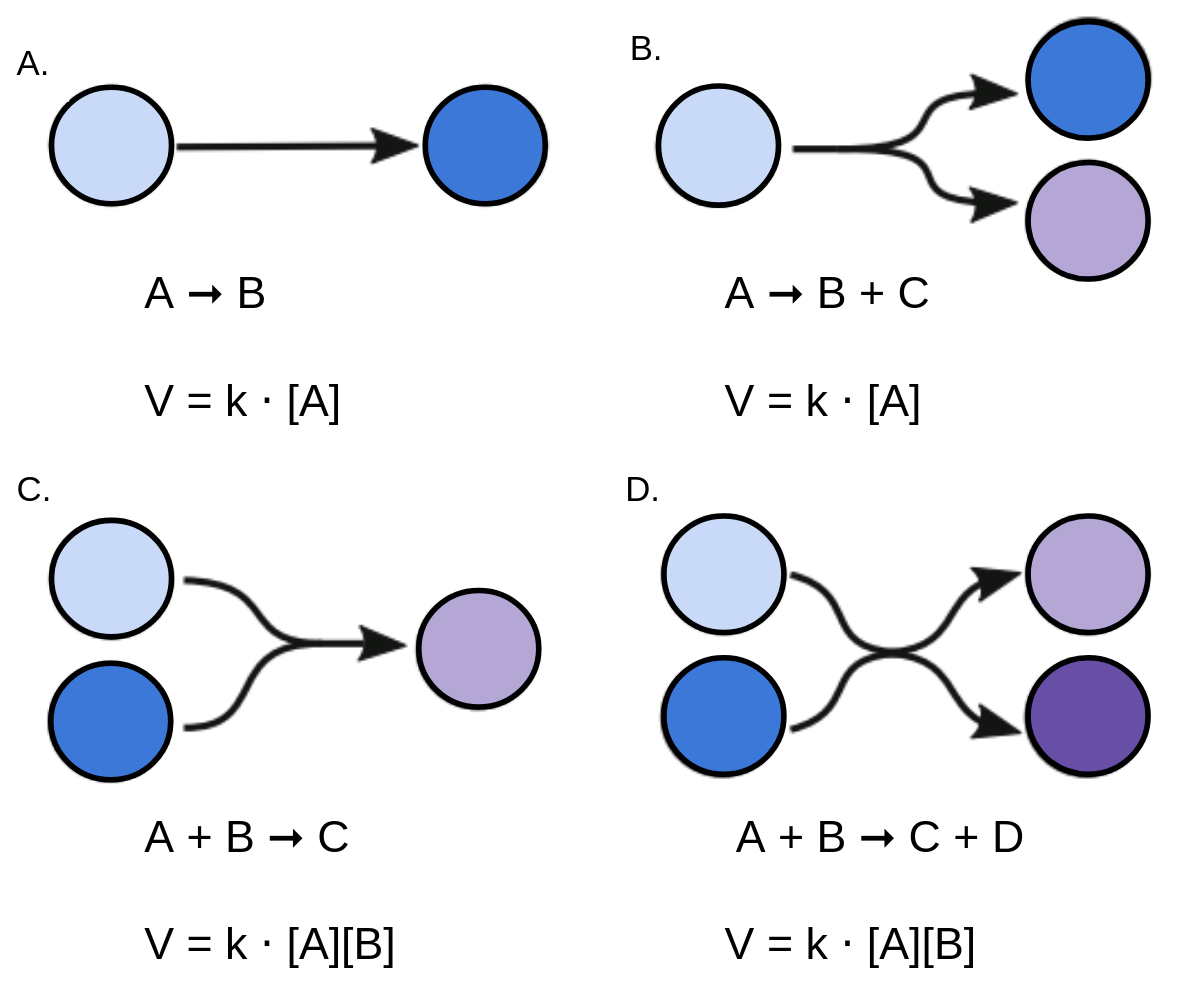
\includegraphics[width=10cm]{images/Reactions.png}
    \caption[Types of reactions and their rate laws]{Models were composed of four reaction types and rate laws: (A) uni-uni, (B) uni-bi, (C) bi-uni, (D) bi-bi}
    \label{fig:reaction}
    
\end{figure}





\subsection{Model Representation}

Models and reactions were represented by custom data structures. An instance of the \textit{reaction} object represents a single reaction and consists of one or two reactants, one or two products, a rate constant, and an integer representing the reaction type (uni-uni, uni-bi, bi-uni, or bi-bi). The \textit{model} object represents a single reaction network and consists of a list of species, a list of initial concentrations, and a list of \textit{reaction} objects. The software converts \textit{model} objects into systems of ordinary differential equations which are then numerically solved to produce time series data of species concentrations. After the evolution process is complete, the models are converted to antimony~\cite{Smith2009}, a human readable model definition language.

\subsection{Objective Function}

The objective function minimized error between the candidate model's time course data and a series of points corresponding to the peaks and troughs of an oscillator. This "idealized" oscillator time series consisted of nine concentration points, alternating between 5 and 30 concentration units over the course of 1.25 seconds (figure \ref{fig:fitness}). The output time series of each species was compared to these points by summing the squared difference between the observed point and the ``ideal" point and the smallest error value was considered the model's fitness. This is similar to MSE but the sum is not divided by the number of observations as this number is constant across all models. This has been demonstrated to be an effective objective function for the in silico evolution of chemical oscillators~\cite{Paladugu2006}.  In cases where candidate models could not be simulated, an arbitrarily high fitness value was assigned resulting in their subsequent removal from the population in the selection step.  

\begin{figure}
    \centering
    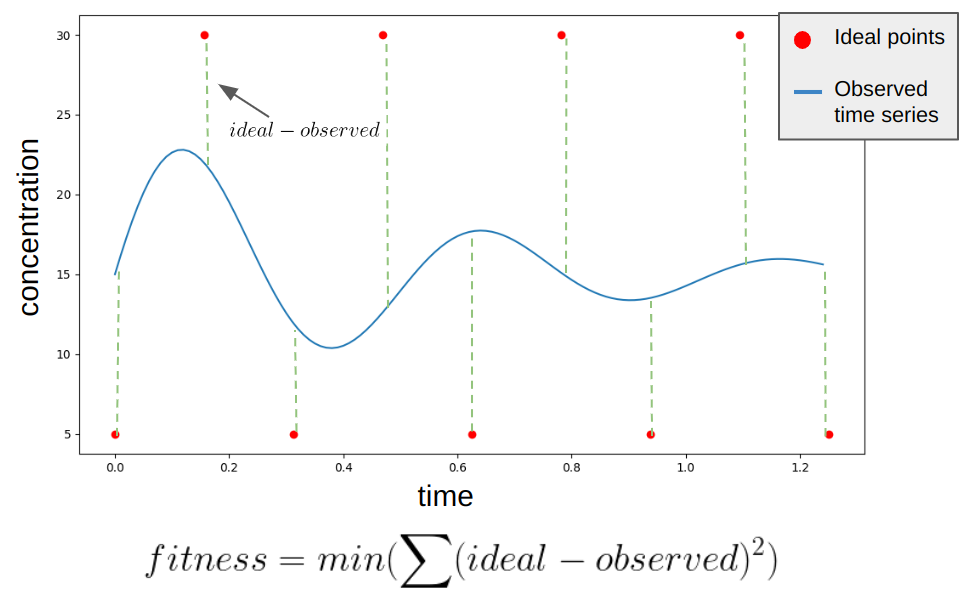
\includegraphics[width=15cm]{images/fitness.png}
    \caption[Oscillator objective function]{For the time series data of this species, the error is calculated by summing the square difference between the observed time series data (blue) and a set of idealized oscillator points (red). This process is repeated for each species in the model and the fitness is defined as the minimum of these sums. }
    \label{fig:fitness}
\end{figure}

\subsection{ODE Solver}
Preliminary studies suggested that the most commonly used python ODE solver from scikit was inaccurate for solving these problems. Other off-the-shelf solvers lacked the ability to deal with the custom data structure encoding the models. The Sauro Lab's simulation software, RoadRunner~\cite{Somogyi2015}, was also unsuitable for this purpose due to the computational cost of frequently modifying and recompiling models for simulation. Many algorithms, such as RK4 are not robust enough for this work. For this reason, a custom simulator using the CVODE solver from the Sundials suite was used~\cite{hindmarsh2005sundials}. 

\subsection{Selection}
In each new generation, the top 10\% of models from the previous generation were copied without modification. The remainder of the new population was chosen by tournament selection~\cite{Miller1995} from the previous generation. This is where two models are randomly chosen from the previous generation (including from the top 10\% of models already carried over) and the model with the better fitness is mutated by adding or deleting a reaction, or by modifying a rate constant. The modified model is then appended to the new generation. 

\subsection{Mutation}
After tournament selection, the fitter model was either mutated by modifying a rate constant or adding/deleting a reaction with equal probability. In the case of rate constant modification, a random rate constant was adjusted by a random percentage between -15\% and +15\% of the rate constant's current value. This mechanism ensured that rate constants could not become negative, and there was no upper limit to their value. 

In the case of reaction modification, a reaction was either added or deleted with 50\%-50\% probability. If deleted was selected, a random reaction was removed from the model. If addition, a new reaction was added with the equal probability of each reaction type: uni-uni, uni-bi, bi-uni, bi-bi (figure~\ref{fig:reaction}). 

\subsection{Random Networks for Evolution}
A population of 40 random networks were generated using the {\tt teUtils} python package~\cite{SauroteUtils_2020}. Each network was initialized with three species, and nine reactions with the probability of each reaction type being 0.1, 0.4, 0.4, 0.1 for uni-uni, uni-bi, bi-uni, and bi-bi reactions. These settings were chosen to maximize the number of evolution trials that successfully product oscillators. All reactions had mass-action kinetics with a random rate constant between 0 and 50. 
\begin{figure}
\begin{center}
    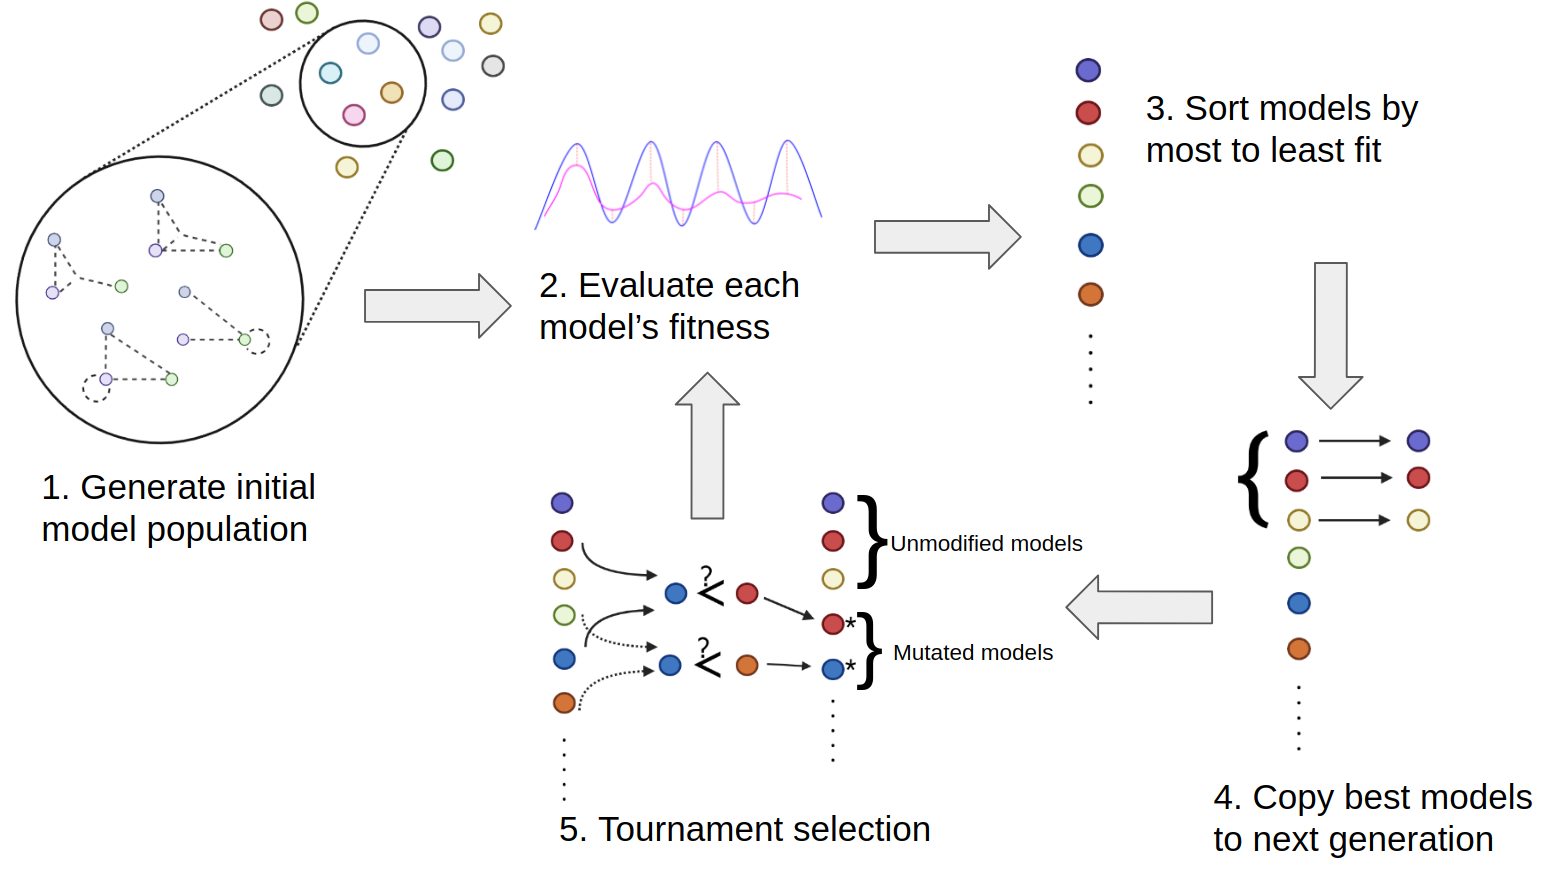
\includegraphics[width=17cm]{images/algorithm.png}
    \caption[Overview of the evolution algorithm in Python]{The evolution algorithm. (1) An initial population of random models is created. (2) The fitness of each model is evaluated. (3) The entire population is sorted by most fit to least fit. (4) The top 10\% of the models are transferred to the subsequent generation unmodified. (5)  Tournament selection is used to populate the remainder of the subsequent generation. Models are randomly selected, the more fit model is chosen to be modified and carried over to the subsequent generation. Steps 2-5 are repeated. }
    \label{fig:algorithm}
    \end{center}
\end{figure}

\subsection{Custom Evolution Algorithm}

The evolutionary algorithm mimics biological evolution in that populations of individuals, in this case candidate networks, are altered and forced to compete with each other. Over the course of generations, fitter individuals (models that oscillate or are likely to oscillate) out compete unfit individuals (models that do not oscillate or can not be simulated) and survive into the next generation. Although genetic and evolutionary algorithms are well characterized, their application to systems biology models remains a challenge as a key trait in these algorithms is crossover, the ability of two possible solutions to exchange information, creating a new, ideally more suitable, candidate solution~\cite{Katoch2020}. Typically, genetic algorithms operate on objective functions for which solutions consist of vectors where values can easily be exchanged between two vectors. It is uncertain how crossover of mass-action kinetic models could be achieved as solutions (candidate networks) consist both of topology (how reactions are connected) as well as rate constants (vectors of values). Additionally, the number of reactions and rate constants vary and must be equal but can vary from model to model. For this reason, a custom optimization process was developed based on genetic algorithms but avoiding crossover. 

This process begins with the generation of 40 random networks with pre-specified probabilities for each of the four reaction types.  The fitness of each model is evaluated by comparing the model's time series data with an objective function representing the desired outcome, oscillation. Models that with time series data close to this desired outcome, those that oscillate or those with damped oscillations, are more fit than those that fail to oscillate or cannot be simulated. 

These models are ordered from most to least fit and the top 10\% of the models are carried over unmodified to the subsequent generation (figure \ref{fig:algorithm}). The remaining models are randomly paired and compared and the fitter of the two models is slightly modified by either adding or deleting a reaction or changing a rate constant. If the modification improves the fitness of the model, the modified model is added to the next generation. If the modification makes the model less fit, 75\% of the time the unmodified model is added to the next generation and 25\% of the time the less fit model will be added. This allows for the chance that small changes initially make a model worse, but subsequent changes drastically improve the model. Once the new generation is fully populated, the models are again ordered from most to least fit and the process begins again. This is repeated for 400 generations or until a threshold fitness level is reached.

\subsection{Random Control Networks}
Random models were generated as described in the previous section. To control for changes made during evolution, the random models underwent the same mutation processes described previously. Instead of populating subsequent generations based on model fitness, 10\% of the previous population was randomly selected to be carried over unmodified to the new generation. The remainder of the new generation was populated with models randomly chosen and mutated from the previous generation. The purpose of this procedure was to account for model variability introduced in the evolutionary process. Of 1000 random control networks generated, 1 was a spontaneous oscillator.

\section{Results}
Evolved models are processed to remove any undesirable oscillators from the population, namely oscillators that dampen over time or oscillators where one or more species concentrations rise indefinitely towards infinity. Next,  duplicated reactions were fused and reactions that are superfluous to oscillation are deleted to minimize network size resulting in a population of reaction networks that oscillate indefinitely in species concentration, examples of which are shown in figure 4.

\begin{figure}
    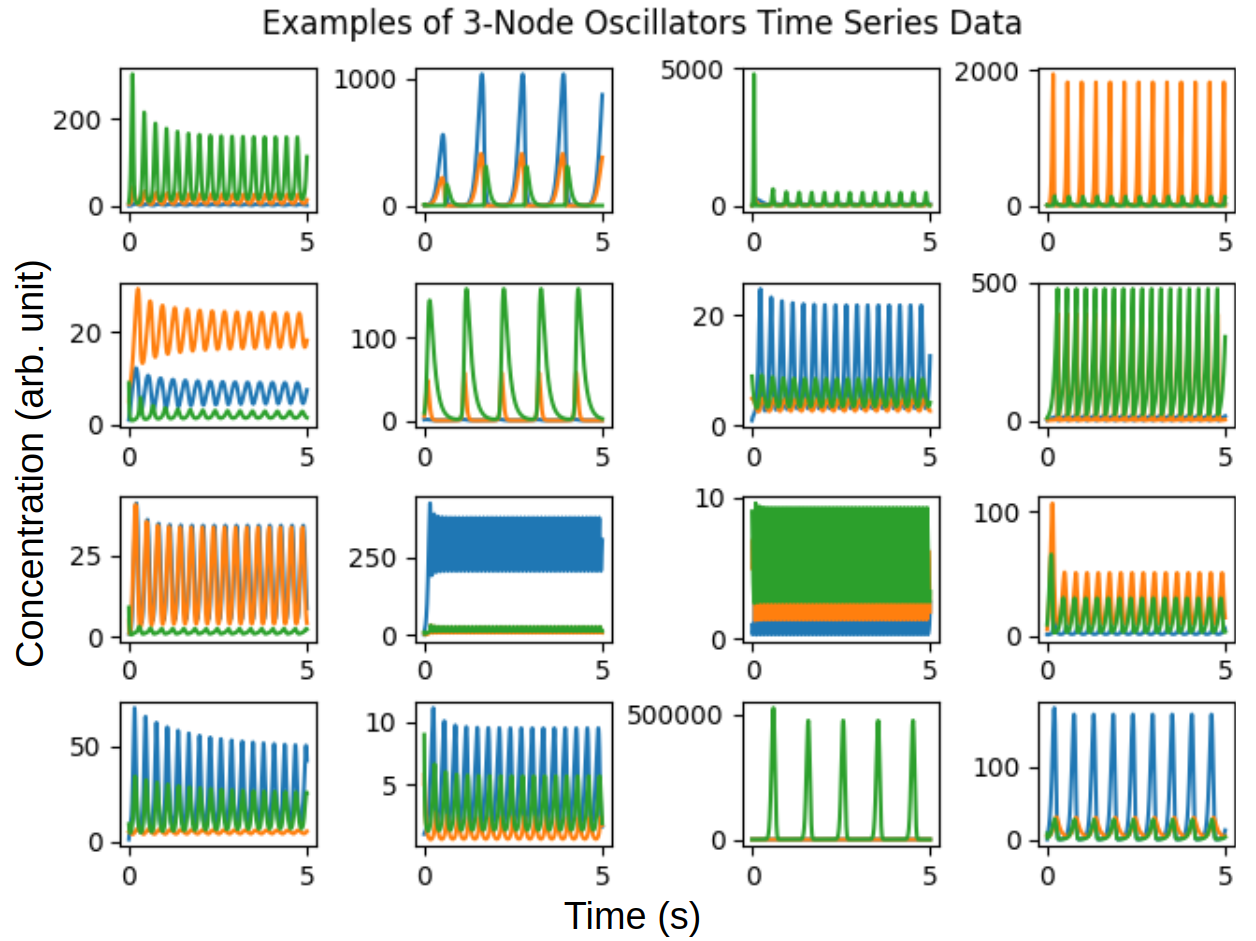
\includegraphics[width=15cm]{images/examples.png}
    \label{fig:examples}
    \caption[Examples of oscillator time series data]{Time series data of sixteen 3-node oscillators generated using differential evolution.}
\end{figure}


\subsection{Database Construction}
A non-relational key-value database was deployed via Mongo Atlas using the PyMongo API to store all models and their information. The user enters the desired reaction network attributes into the web GUI (figure \ref{fig:website}). Models are downloaded as a .zip file of text files, or if a single model a single text file, containing the antimony string of each model. If the "Download in simulatable Tellurium form" box is checked, then each model file will contain the necessary python package imports and formatting to be immediately simulated and plotted upon running the file.


The current website queries the database by model type (current options are oscillator or random), the number of nodes (species), the number of reactions, and the presence or absence of autocatalysis or degradation reactions. Both oscillator and non-oscillating control networks are stored in the database. Each entry also includes a dictionary of tallies of each reaction type in the network, a list of redundant reactions that were fused during post-processing, a list of reactions that were deleted as their presence did not influence oscillation. 




In addition to the Antimony string comprising the model, other characteristics such as its initial reaction probabilities, fused and deleted reactions, and reaction counts are also tracked in the database.  The database can be queried to select models with any number of desired traits. Both oscillator and non-oscillating control networks are stored in the database.

The Cesium database is publicly available on the web at \url{https://cesiumdb.herokuapp.com/} and is intended to serve as source of reaction networks with specified characteristics for use in research and validation.  It currently contains 2000 randomly generated models and approximately 1800 3-species oscillating networks. This database can be expanded in the future to include a wider variety of oscillatory networks as well as networks with different behaviors, such as bistability. 

\begin{figure}
    \centering
    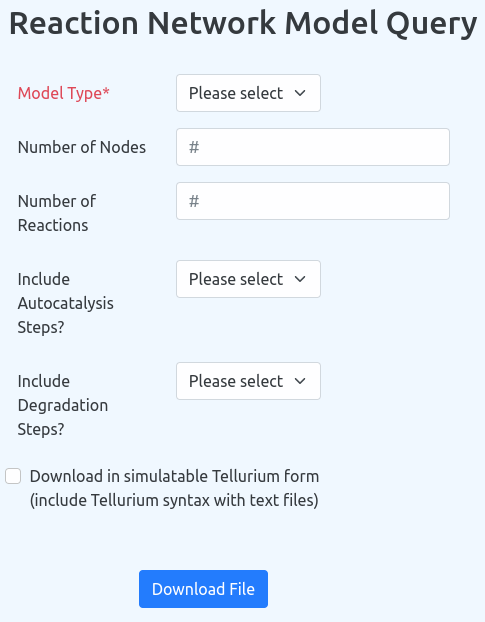
\includegraphics[width=12cm]{images/website.png}
    \caption[Landing page for the Cesium database website]{Landing page for the Cesium database.}
    \label{fig:website}
\end{figure}

\subsection{Oscillating Network Examples}
Four oscillating networks from the database are shown in figure \ref{fig:model-diagrams}. Arrows symbolize reaction and lead from the reactant to the product. A double headed arrow indicates two products are formed and a double tail indicates two reactants. 


\begin{figure}
    \centering
    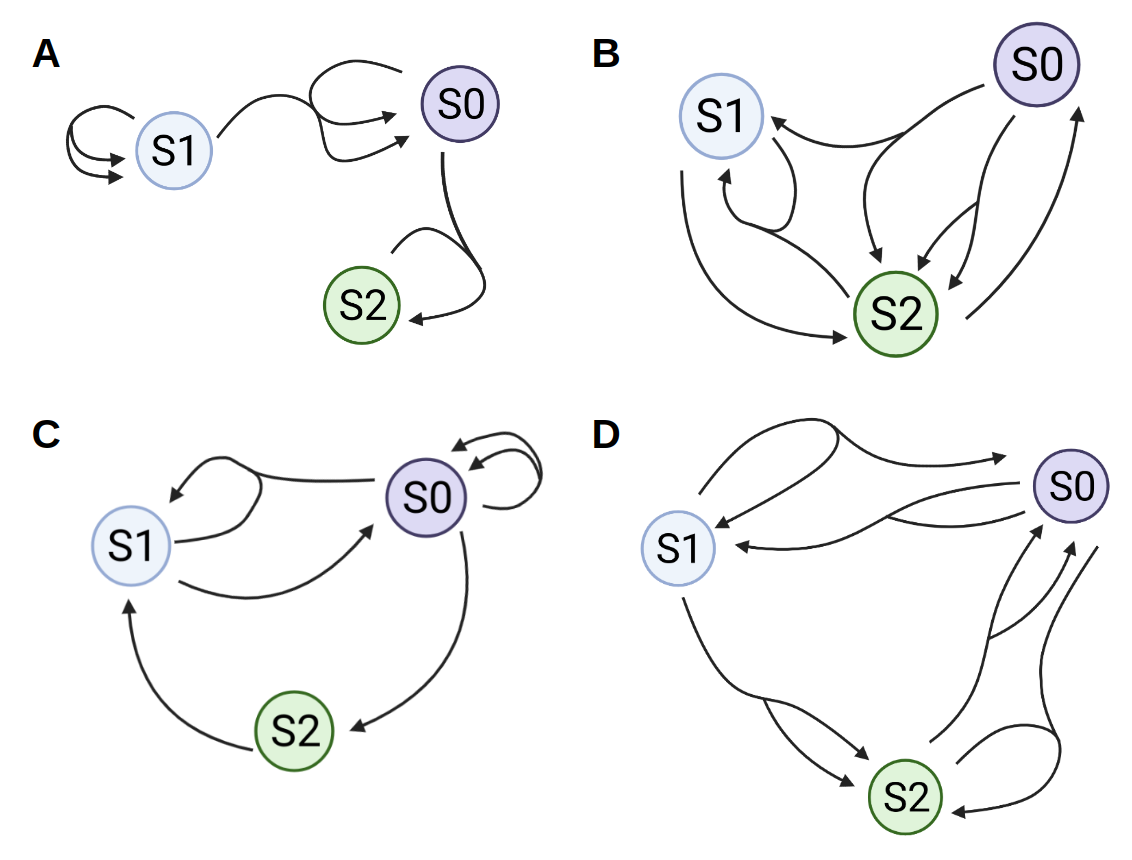
\includegraphics[width=12cm]{images/model-diagrams.png}
    \caption[Examples of evolved oscillating networks]{Examples of 3-species oscillating networks from the Cesium database.}
    \label{fig:model-diagrams}
\end{figure}

In network A, S1 is autocatalytic as is S0 (and catalyzed by S1). These linked positive feedback loops cause oscillation with products out flowing to S2, which essentially behaves as a boundary species, a species that is unaffected by the model and whose concentration remains fixed.  Network B lacks autocatalytic reactions completely. Computing the jacobian matrix at the unstable focus results in the following matrix:
\[
\begin{blockarray}{cccc}
S0 & S1 & S2 \\
\begin{block}{(ccc)c}
  -4.75 & 0 & 15.2 & S0 \\
  0.75 & -0.3 & 0 & S1 \\
  8.75 & -1.6 & -22.8 & S2 \\
\end{block}
\end{blockarray}
 \]
In the bottom row center, the negative number indicates that there is an inhibitory relationship between S1 and S2. An increase in S2 will decrease the production rate of S1. These interactions for a cycle with negative feedback, suggesting that this is a feedback oscillator (figure \ref{fig:feedback}). Similar analyses reveal that networks C and D are also likely to be feedback oscillators.

\begin{figure}
	\centering
    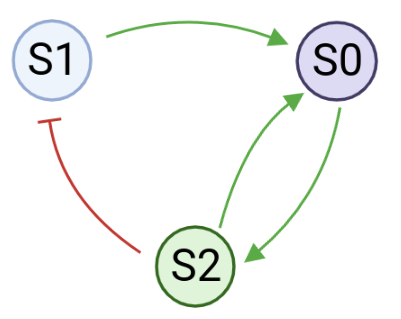
\includegraphics[width=8cm]{images/feedback-cycle.png}
    \caption[Feedback diagram of an oscillating network]{Species interactions of Network B. Green arrows indicate activation and blunt red arrows indicate inhibition. The interactions form a cycle with negative feedback suggesting that Network B is a feedback oscillator.}
    \label{fig:feedback}
\end{figure}


\section{Discussion}

Oscillating models were significantly enriched for autocatalytic reactions compared to control networks. Most oscillators are associated with unstable steady states. Destabilizing processes can be classified as 1) direct autocatalysis, 2) indirect autocatalysis (a positive feedback loop), and 3) end-product inhibition (a negative feedback loop)~\cite{Tyson1975, tyson2007}. Reactions are considered autocatalytic when the products increase the rate of reaction or when a chemical decelerates the rate of its own destruction~\cite{Tyson2004}. Given the two types of oscillators, negative feedback and negative feedback coupled with positive feedback~\cite{Sauro_dynamics}, it is unsurprising that autocatalytic reactions are enriched in the oscillator population as these reactions are a form of positive feedback. The portion of models containing at least one autocatalytic reaction in the oscillator and control populations were compared using a two-way chi square test. Of the 586 oscillating models, 83.1\% (487 of 586) contained an autocatalytic reaction compared with 49.8\% (498 of 1000) of the control models, a significant difference ($p < 0.0001$). 

Given the enrichment of autocatalytic reactions, one might expect a similar enrichment of degradation reactions, reactions where one species is removed from the system (eg. $X + Y \to Y$, where $X$ is removed from the system), to prevent species concentrations from rising to infinity. Interestingly, the presence of degradation reactions were not enriched in oscillating models. Of the oscillating model population 79.4\% (465 of 586) contained at least one degradation reaction compared to 76.3\% (763 of 1000) of the control models, an insignificant difference suggesting that although autocatalysis is a common characteristic in oscillating networks, degradation reactions are not necessary to prevent species concentrations from rising to infinity.  Although the presence of both an autocatalytic and a degradation reaction are not necessary for oscillation, it is rare that an oscillator contains neither. Only 0.5\% (3 of 586) of the oscillators analyzed had neither an autocatalytic reaction nor a degradation reaction compared to 0.2\% (2 of 1000) random models, an insignificant difference.

To determine if any reaction types were enriched in the oscillator population compared to the control population, the average model compositions were compared. The average model composition was assessed as the average number of reactions of the specific type were divided by the average total number of reactions for each group. For example, there were an average of 6.592 reactions per model in the oscillator population, of which an average of 0.99 were uni-uni reactions, for an average of 15.3\% uni-uni reactions in the average oscillator model (Table \ref{fig:avg-comp}). Compositions were compared with permutation tests, showing that model compositions and sizes were significantly different between the oscillator and control populations (the reduced size of oscillating networks can be accounted for by the fusion of duplicate reactions). Oscillators possessed significantly more uni-bi reactions compared to random control models. This is consistent with the enrichment of autocatalytic reactions which are often uni-bi. However, autocatalytic reactions can also be bi-bi reactions, which were not enriched in oscillating models. Although bi-bi reactions were less likely to be created during evolution due to the initial settings (10\%), it is somewhat surprising that bi-bi reactions were decreased in oscillatory networks given that a bi-bi reaction is slightly more likely to be autocatalytic ($\frac{4}{27}$) compared to a uni-bi reaction ($\frac{1}{9}$).

\begin{table}
	\centering
    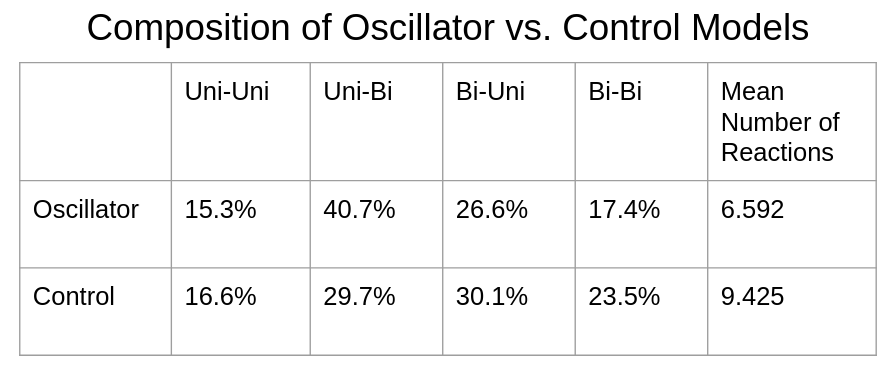
\includegraphics[width=12cm]{images/composition.png}
    \caption[Composition of oscillator vs. control models]{Average reaction compositions of oscillating networks compared to non-oscillating controls.}
    \label{fig:avg-comp}
\end{table}

Next, oscillators containing autocatalytic reactions (498 models) were compared to oscillators lacking them (98 models). Populations were compared by permutation test. There was a significant increase in the portion of uni-bi reactions and a significant decrease in the portion of bi-uni reactions in non-autocatalytic models as compared to autocatalytic oscillators (Table \ref{fig:autocatal}). This result is interesting given that autocatalytic reactions are either uni-bi or bi-bi and both reaction types were reduced in oscillators with autocatalytic reactions compared to oscillators without. It is possible that oscillators without a single autocatalytic reaction are achieving autocatalysis through a combination of non-autocatalytic reactions.

\begin{table}
	\centering
    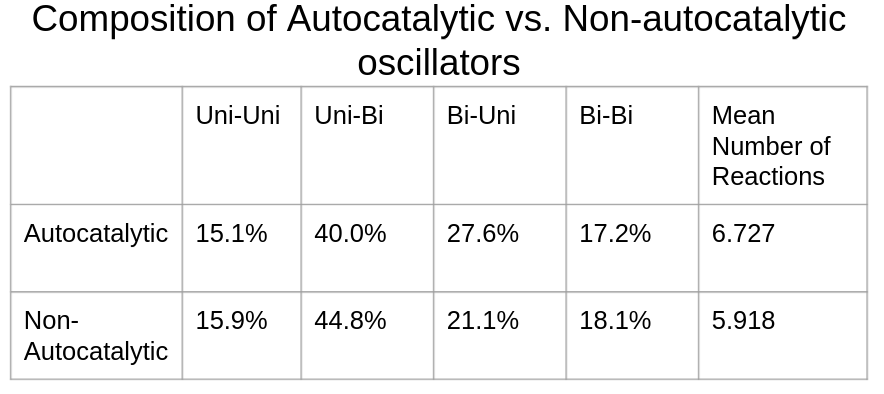
\includegraphics[width=12cm]{images/autocomp.png}
    \caption[Composition of autocatalyitic vs. non autocatalytic oscillators]{Average reaction compositions of autocatalytic oscillating networks compared to non-autocatalytic oscillating networks.}
    \label{fig:autocatal}
\end{table}

Several manually inspected oscillators had reactions with extremely high rate constants (greater than 300, whereas most rate constants were between 5 and 75). The initial range for rate constants is 0 to 50 and with each mutation, they can only increase a maximum of 15\% of the current value. Although there is no upper limit for rate constants, it is nearly impossible to mutate a rate constant from the initial range to over 100 during the course of evolution. To bypass this limit and achieve high rate constants, many successful models have simply duplicated reactions during the evolutionary process. During post-processing, these duplicate reactions are fused and their rate constants summed. Fusing duplicate reactions to achieve high rate constants accounts for the observation that oscillators generally have fewer reactions than non-oscillators in this study. These high rate constant reactions can not be removed, nor can the rate constant be significantly lowered without impacting oscillation. Further investigation is needed to determine what essential function these high rate reactions seem to play in most of the oscillators included in this study. 


These oscillatory models and the random control networks have been added to a database, accessible at \url{https://cesiumdb.herokuapp.com/}. Models can easily be selected by the number of species, the number of reactions, and the present of autocatalysis or degradation reactions. The selected models can be downloaded in a zip file containing a .txt for each model. Each .txt file contains an individual model's antimony string. If the "Download in simulatable Tellurium form" option is selected, the .txt file will also contain formatting and package imports allowing the model to be easily simulated when the file is run as a python script. 

In the future, this database will be expanded to contain a variety of models with different behaviors besides oscillation. It is our hope that this database serves as a resource for the modeling community to study network behaviors and test novel software.


\section*{Funding}
This project was supported by National Institute of Health grant U01 CA238475 and the National Institute of Biomedical Imaging and Bioengineering for grant P41GM109824.

\section*{Acknowledgements}
We thank Lucian Smith for valuable discussions on differential evolution and model topology. 
\\
\\
This chapter was adapted from the following publication:
\\
\textbf{Tatka, L.}, Luk, W., Hellerstein, Elston, T., J., Sauro, H. “Cesium: A Public Database of Evolved Oscillatory Reaction Networks.”  Biosystems, vol. 224, 2023, p.104836., \\
https://doi.org/10.1016/j.biosystems.2023.104836. 
\\


\chapter{In Silico Speciated Evolution of Oscillatory Mass-Action Reaction Networks}
\label{chap: NetEvolve}
\section{Introduction}
Genetic algorithms (GAs), inspired by the principles of natural selection and genetics, have emerged as a powerful computational technique for solving optimization and search problems.Developed by John Holland in the 1970s, GAs mimic the process of biological evolution to solve optimization and search problems \cite{holland_1975}. At their core, genetic algorithms operate on a population of potential solutions, represented as individuals or ``chromosomes," each encoding a candidate solution to the problem at hand. Through iterative generations, genetic algorithms apply mechanisms of selection, crossover, and mutation to evolve and refine the population, gradually converging towards optimal or near-optimal solutions. Selection favors individuals with higher fitness, mirroring the process of natural selection, while crossover and mutation introduce variation and diversity into the population, allowing for exploration of the solution space. By leveraging the principles of evolution, genetic algorithms offer a versatile and robust approach to solving complex problems across various domains, from engineering and optimization to biology and beyond.

A key feature of genetic algorithms is crossover, the exchange of multiple parameters between two candidate solutions to create a new offspring solution. Crossover proves challenging when solutions are not vectors of matrices of numbers, but also include graphs. Stanley and  Miikkulainen devised a method, NEAT, to crossover topologies when evolving artificial neural networks. Dinh et al. adapted NEAT to enable crossover when evolving gene regulatory networks. Here, the NEAT algorithm is adapted and explored with mass-action chemical reaction networks. In contrast to previous studies in different domains, the crossover method presented here does slightly reduces the success rate of evolution. 

Speciation, though not essential to evolutionary algorithms, can improve their success by protecting innovations and allowing them time to develop into better solutions. This work also introduces a method for separating chemical reaction networks into species and explores the effect of speciation on evolutionary success. Separating similar chemical reaction networks into species significantly improves the sucess of the algorithm.

\textbf{Some stuff about speciation}

The purpose of this work it twofold: (1) to create a general purpose, easily customizable, module for evolving mass-action chemical reaction networks and (2) to explore the effects of crossover, speciation, and other hyperparameters on the success rate of the algorithm. Speciation is found to be essential to the success of the algorithm. In contrast to previous studies in different domains, the crossover method presented here does slightly reduces the success rate of evolution. 


In addition to speciation and crossover, a variety of evolutionary hyperparameters are explored in evolving oscillatory mass-action networks. The evolutionary algorithm is packaged in a library written in the julia programming language \cite{bezanson2017julia}. It is highly configurable and allows users to easily specify settings via the command line for a simple json file. It can generate reaction networks to match a variety of time series data beyond oscillators.




\section{Evolving Reaction Networks}
The purpose of this work it twofold: (1) to create a general purpose, easily customizable, module for evolving mass-action chemical reaction networks and (2) to explore the effects of crossover,  speciation, and other hyperparameters on the success rate of the algorithm. Oscillatory chemical reaction networks were chosen as the target result of the evolutionary algorithm due to their biological relevance, poorly understood architectures (maybe??), and the presence of intermediary states (damped oscillations) which aids in gradual evolution.
----

Oscillatory behavior is useful in a variety of biological processes including p53, circadian rhythm, and cell cycle. But also, you might want to generate oscillators as a component in a syntehtic biology ciruit. But really, this isn't about oscillators, that's just the test case. You might want a certain behavior and don't know how to build a  network to get it. Well This algorithm is for you! 

Other people have done similar things, but this is different. It starts with the concept of genetic algorithms, way back in 1975. These are algorithms to come up with optimization solutions. The algorithms kind of look like biologic evolution. You have a bunch of individuals, the fitter individuals share their genes and reproduce, less fit individuals die off, sometimes mutations occur and these can be either good or bad. Since then, the concept of genetic algorithms has been thoroughly explored, but here we present something slightly new. And that's how I'm going to get my PhD lol.

This all starts with the NEAT algorithm which is a way of evolving neural networks to do stuff.  What's interesting about this is they claim to have meaningful crossover and they use speciation to protect innovation. Dinh et al somehwat adapted this appraoch to genetic circuits, but those are a much easier problem because they just have activation and inhibition. Here, I adapt this algorthim to mass-action networks. That's way harder because there is way more complexity. In the first case, you just have an edge that connects two nodes and a weight. In the second, you add that the edge can either be activating or inhibiting, but here we add that the edge could connect multiple nodes (in the case of everything beyond a uni-uni reaction) and the reaction weight depends on what nodes it connects. More on that later.

I need to go over a bunch of times that this was done for a similar thing. Just as a quick review




\section{Methods}

\begin{figure}
\centering
    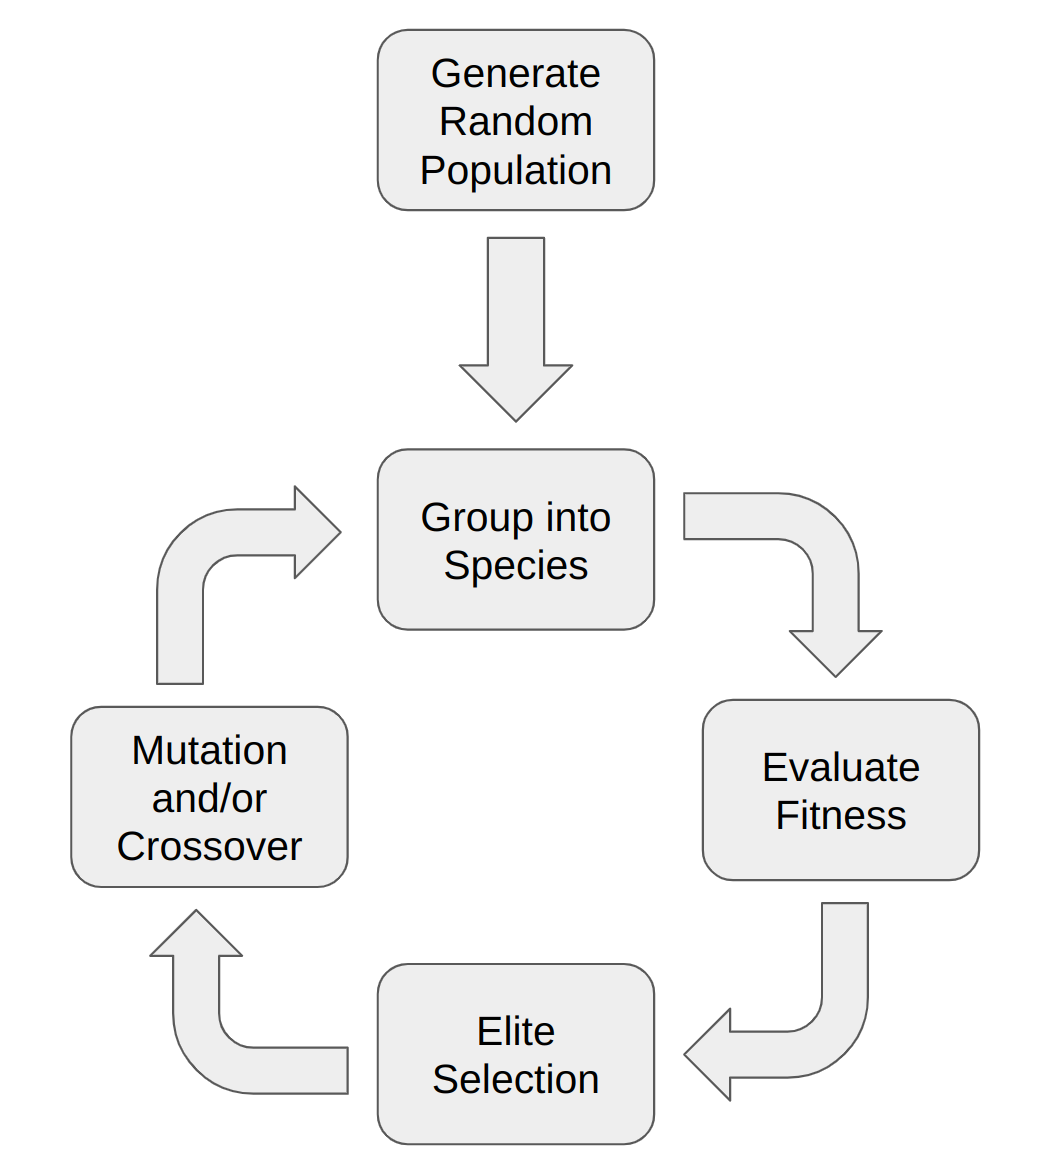
\includegraphics[width=8cm]{images/algo_description_crossover.png}
    \caption[Overview of the evolution algorithm with speciation]{The evolutionary algorithm begins with a population of randomly generated reaction networks. These networks are then grouped into species and their fitness evaluated. The next generation is constructed by first selecting the top performing individuals from each species without modification. The rest of the subsequent generation is populated by networks that are modified by either crossover, mutation, or both. This new generation is then grouped into species based on structural similarity and the process repeats.}
    \label{fig:algo_description_crossover}
\end{figure}


\subsection{Encoding}
Chemical reactions are represented as custom data structures that contain one or two reactants, one or two products, a rate constant, and a boolean value indicating if the reaction is active or inactive. Four types of mass-action reaction are possible: uni-uni (a single reactant to a single product), bi-uni (two reactants form a single product), uni-bi, and bi-bi. A reaction that is active participates in the network that it is part of. An inactive reaction is ``turned off" but remains part of the network as a historical record. It can be activated again or crossed over under certain circumstances. 

A reaction network is a custom data structure consisting of several reactions, initial concentrations for the floating species, and other information to track the individual network. A network can include boundary species (which are assumed to be at a constant concentration throughout the simulation), but boundary species were not used in this study.

\subsection{Mutation}
\label{section: mutation}
There are two types of mutation: rate constant mutation and reaction addition or subtraction. The probability of each of these mutations occurring and the range in which rate constants are mutated can be set by the user. A rate constant mutation can occur in two possible forms. The rate can be increased or reduce by a random percentage, uniformly distributed in a custom range (by default $\pm20\%$), or more rarely a completely new rate constant can be selected, uniformly distributed within a custom range (by default 0.1 to 50). Rate constants were not allowed to become negative, but they did not have an upper bound as previous studies observed that many synthetic oscillating systems rely on a single reaction with an abnormally large rate constant \cite{Tatka2023}.

A reaction mutation is either the addition of a new random reaction or the deletion of an existing reaction, with 50\% chance of each. When a new reaction is added, it is generated randomly with a 
probability of 0.1, 0.4, 0.4, 0.1 for uni-uni, uni-bi, bi-uni, and bi-bi reactions respectively. These probabilities are also configurable. If the randomly generated reaction is already present in the reaction network, the new reaction's rate constant is added to the existing reaction's rate constant. This feature can allow some rate constants to grow to several multiples of the next largest rate constant in the network. When a reaction is deleted, it is ``switched off" and becomes inactive in the network, but is preserved as it can become reactivated under certain circumstances.

\subsection{Crossover}
\label{section:crossover}
During crossover, two parent networks from the same species group are chosen to mate. Analogous to natural evolution, crossover is essential a means of changing more parameters simultaneously and to a greater degree. It injects for novelty into the offspring network compared to single mutations. This could either result in faster progress towards a good solution, or could interrupt progress by destroying decent solutions.

Crossover occurs by examining each reaction in the parent networks. If a reaction is present in both parents, the reaction will be passed down to the offspring network with the rate constant randomly chosen from one parent. If a reaction is present in the more fit parent, but not the less fit parent, the offspring network will inherit the reaction. If an inherited reaction is currently inactive meaning it was previously deleted during a mutation step), there is a 0.25 probability of the reaction becoming active again. If both parents are equally fit, one is randomly chosen to be the more fit parent (table \ref{table:crossover_table}). 

\begin{table}
	\centering
    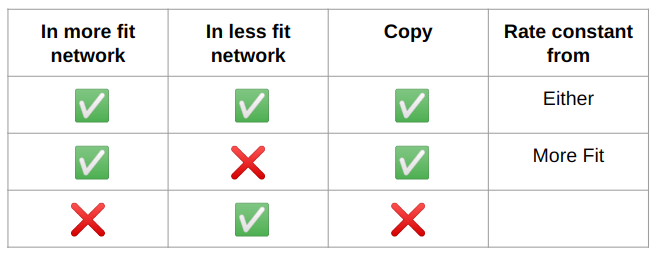
\includegraphics[width=12cm]{images/crossover_table.png}
    \caption[Crossover procedure]{Every reaction in the more fit network is passed down to the offspring network. If it occurs in both parent networks, the rate constant is randomly inherited from one parent or the other.}
    \label{table:crossover_table}
\end{table}

A second crossover strategy for similar networks was tested in later trials. Networks that were members of the same species and had similar fitness score (within 5\% of each other) underwent a slightly different crossover process. All reactions that the two networks had in common were passed down to the offspring network with rate constants chosen randomly from one parent or the other. Reactions that occurred in one parent network but not the other had a 50\% chance of being passed down to the offspring network.

\subsection{Speciation}
In many cases, modifying a network, especially through the addition or deletion of reactions, initially makes the system less fit. Without speciation, these innovations seldom last for more than a generation. However, often these topological innovations prove an essential step in evolution \cite{stanley_evolving_2002}. For this reason, a speciation strategy is employed to protect innovations and allow them time to optimize. Individuals with similar topologies are grouped into species. Members of a species compete only with each other and not the population at large.  A compatibility distance metric, $\delta$, is used to assign reaction networks to a species, defined as

\begin{equation}
\delta=\frac{M}{N}
\end{equation}
where M is the number of reactions in the larger network that are not present in the smaller network and N is the total number of reactions in the larger network. Two reactions are considered identical if they have the same reactants and products. Rate constants are not considered. If $\delta$ is below the speciation threshold, $\delta_{t}$, the two networks are members of the same species.

For each new generation, networks are assigned to species based on the previous generation's species groups. Each new network is compared to a randomly chosen individual from a species in the previous generation. If $\delta$ is less than the speciation threshold $\delta_{t}$, then the network is assigned to that species. If $\delta$ is greater than $\delta_{t}$, then the network is compared to a randomly selected individual from the next species, etc., until a match is found. If no species is assigned after comparing the network to all species in the previous generation, then a new species is created. 

The speciation threshold $\delta_{t}$ is adjusted with each generation to steer the total number of species towards the target number of species. The target number of species is 10 by default, but can be configured by the user. After each generation the total number of species is counted. If there are more species than the target value, $\delta_{t}$ is increased allowing networks that are more dissimilar to be grouped together. If there are fewer species than the target value, $\delta_{t}$ is decreased. Adapting $\delta_{t}$ as evolution proceeds maintains an optimal number of species. If there are too many species each with a small number of members, there are not enough opportunities to optimize solutions in a small parameter space. Similarly, if there are too few species with several members, the entire parameter space is not adequately explored. 

\begin{equation}
	\delta_{t} = \begin{cases}\delta+\epsilon,& \mbox{if number of species} > N_{s} \\
	\delta-\epsilon,& \mbox{if number of species} < N_{s}
	\end{cases}
\end{equation}

\subsection{Objective Function}

The objective function evaluated how well a candidate model oscillated at the imposed time period, $T$.  Two arbitrary concentrations, $[C]_{1}$ and $[C]_{2}$,  were chosen \textit{a priori}. The fitness score of a particular network was then attributes to how well any of its chemical species approached $[C]_{1}$ at half periods ($T/2$, $3T/2$, $5T/2$,...) and  $[C]_{2}$ at each period ($T$, $2T$, $3T$,...) over the course of 5.5 periods. The candidate model's single chemical species that best approached these points was selected and the fitness was evaluated as the maximum of the reciprocal of the absolute difference between the timeseries data and $[C]_{1}$ or $[C]_{2}$, the ``ideal oscillator" time points, (equation \ref{equation: fitness}). The reciprocal was taken so that higher values represented better fitness, which is necessary for determining the number of offspring for each species in subsequent steps. This objective function has been shown to be an effective means of evolving oscillators in similar and previous works \cite{Paladugu2006, francois_hakim_2004, Tatka2023}. In cases where candidate models could not be simulated, a fitness of 0.0 was assigned resulting in the candidate model's subsequent removal from the population.

\begin{equation}
\label{equation: fitness}
fitness = max(\frac{1}{\sum|ideal - candidate|})
\end{equation}

\subsection{ODE Solver}
During the fitness evaluation phase, reaction networks were converted to systems of ordinary differential equations. These equations were then numerically solved using the DifferentialEquations.jl julia package \cite{DifferentialEquations.jl-2017} and the CVODE solver from the Sundials suite for solving initial value problems \cite{hindmarsh2005sundials}. The CVODE solver was shown to be effective for this application in previous work \cite{Tatka2023}.

\subsection{Reproduction}

Each model species was allocated offspring in proportion with its fitness. More fit species were allowed more offspring. To calculate the number of offspring allocated to each species group the sum of fitness values was computed across the entire population. Then each species, $s$, was assigned an offspring number proportional to its contribution to the fitness of the entire population (equation \ref{equation: num_offspring}). Two strategies were tested for assigning species fitness. In one case, species fitness was calculated as the average fitness of the individuals in the species. In the second case, species fitness was the fitness of the best network in the species. The calculated number of offspring for each species was rounded to the nearest integer. By default, a single species was only allowed to produce at most 10\% of the subsequent generation in order to prevent a single species from taking over the entire population (but this value could be adjusted by the user). For these reasons, the total number of individuals fluctuated slightly over time.


\begin{equation}
\label{equation: num_offspring}
offspring_{s} = \frac{\sum{fitness_{s}}}{\sum{fitness_{pop}}}*populationsize
\end{equation} 


The reproduction phase began with an elitism selection strategy. The top 10\% of networks in each species were copied to the next generation directly. If a species had 10 or fewer individuals, the single best network was copied without modification to the next generation. Then, the bottom 10\% of networks in each species are deleted. For the remainder of the allocated offspring for each species, a random number, $p$, was generated. If the $p$ was less than the probability of crossover, then two networks from the same species were selected and crossed over to produce a single offspring network. Otherwise a single network was chosen. If $p$ was greater than or equal to 1 - the probability of mutation, the network was mutated. Outside of the elite networks, all networks were either crossed over or mutated. Some were both crossed over and mutated. The probabilities of crossover and mutation could be configured by the user. Probabilities for specific types of mutations are described in section \ref{section: mutation}.

Tournament selection was also explored and can be configured in settings. In this case, two networks from the same species were randomly chosen and the more fit network was then crossed over, mutated, or both. If crossed over, a second network was also chosen by tournament selection.

\subsection{Output}
The evolutonary aglorithm was repeated for a preset number of generations (800 by defualt) or until the best model reached a predefined fitness level. At this point, the best model from each species was converted to Antimony, a human readable model definition language \cite{Smith2009} and written to a text file along with the model's fitness. All settings were also written out to a JSON file, which could be used without modification to repeat the evolution trial.

The best models from each evolution trial were automatically assessed with a Python script using the Tellurium modeling environment \cite{Choi2018} and RoadRunner simulation software \cite{andy2020}. A model was considered an oscillator if its Eigen values at steady state contained a positive real number with a nonzero imaginary number and if all concentrations were positive at steady state. Models that met the Eigen value criteria but had negative steady state concentrations were flagged. Flagged models then underwent a simple automated repair process wherein each reaction was deleted one at a time in an effort to meet the oscillation criteria. Models that met criteria after the simple repair process were counted as oscillators.

\section{Results}
The software was evaluated with multiple hyperparameter settings to assess its ability to generate oscillatory mass-action chemical reaction networks. Each set of hyperparameters were evaluated over 700 evolutionary trials and the success rate recorded. A trial was deemed successful if it generated a network with sustained oscillations, as evaluated by the criteria described previously.


\subsection{Verifying Speciation}
Before evaluating the effects of speciation on evolution, tests were run to verify that speciation was occurring and that the adaptive $\delta$ threshold was maintaining the target number of species. Batches of 700 trials were run for a target number of 1 (no speciation), 5, 10, 30, and 50 species. Figure \ref{fig:avg_num_species} shows that on average, these target numbers were achieved. During the initial generations, the number of species fluctuates more dramatically. This is like due to the fact that while $\delta$ is adaptive, $\epsilon$, the amount by which $\delta$ is changed, is not. During the first several generations, adjustments to $\delta$ tend to over or under shoot the target number of species, likely due to there being large differences between individual networks at first. This over and undershooting causes the number of species to fluctuate before leveling out to the target level after approximately 15 generations.

\begin{figure}
\centering
    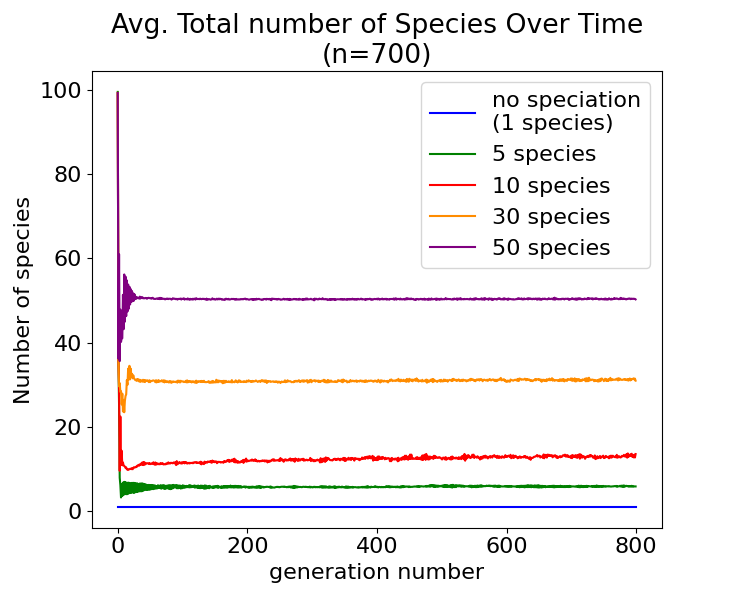
\includegraphics[width=15cm]{images/avg_num_species.png}
    \caption[Average total number of species over time]{Adapting $\delta$ maintains the target number of species without the need to select a value that results in the target number of species through trial and error.}
    \label{fig:avg_num_species}
\end{figure}

The benefit of an adaptive $\delta$ is that the user need only specify the target number of species and $\delta$ will change to accommodate that specification. Without adaptation, $\delta$ must be chosen through trial and error so that it results in the target number of species. For example, in the case of a target species of 10, with an adaptive $\delta$, the total number of species converges to 10 after a few generations and remains there until the end of the trial (figure \ref{fig:adaptive_delta}). With a constant $\delta$, the total number of species is gradually reduced over the course of the trial. In this example, in both cases the success rate was about the same 22\% vs 22.5\% for adaptive and constant $\delta$ respectively. 

\begin{figure}
\centering
    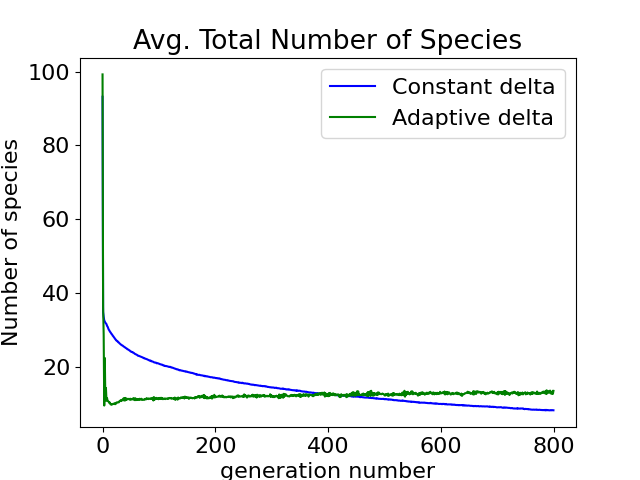
\includegraphics[width=15cm]{images/adaptive_delta.png}
    \caption[Adaptive $\delta$ maintains the target number of species]{Adaptive $\delta$ maintains the target number of species compared to a constant delta.}
    \label{fig:adaptive_delta}
\end{figure}


Although the total number of species remains relatively constant over time, the different species tend to become more similar to each other. The inter-species distance between two species is defined as the distance between the best networks from each species. At each generation, the distance between every combination of 2 species were measured and the average of these measurements recorded. This measurement was performed for batches of 700 trials each for a target of 5, 10, 30, and 50 species. For all four conditions, the average inter-species distance is reduced over time, possibly due to convergence to a single best solution. All three batches started with an average inter-species distance of approximately 0.9, meaning that species differed by an average of 90\% of their reactions. The batch with a target of 10 species converged the most, with an average inter-species difference of approximately 0.55 after 800 generations.   Batches with a target of 30 and 50 species did not converge as much and ended with an average inter-species distance of approximately 0.75 and 0.80 respectively. Larger distances with more species may be due to elitism. With a target of 50 species, at least 50 individuals will be copied to the next generation with no modification. Perhaps lesser networks that otherwise would have been removed if forced to compete with more individuals are allowed to reproduce. Reducing the removal of less fit individuals may allow them to maintain their distances over time. Trials with a target of 5 species converged more rapidly at first, but ultimately did not converge as much as trials with a target of 10 species. Perhaps with too few species, more fit networks dominate the population early on and cause more rapid convergence. However, as evolution progresses, trials with fewer species are less likely to find a good solution and therefor do not further converge.

\begin{figure}
\centering
    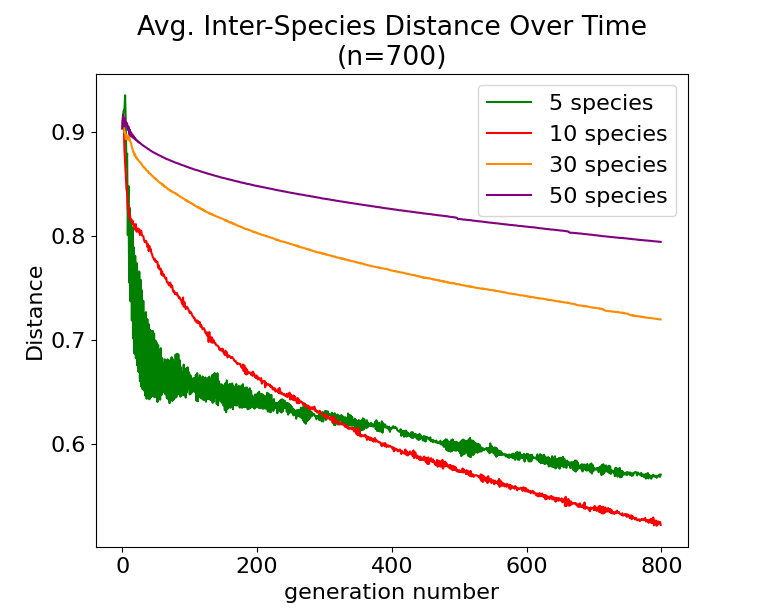
\includegraphics[width=15cm]{images/avg_species_differences.png}
    \caption[Average inter-species distance over time]{Different species become more similar over time.}
    \label{fig:avg_species_differences}
\end{figure}

Next, the average intra-species distances were compared for different target numbers of species. The intra-species distances was computed by averaging the distance between every combination of pairs of networks within a single species. As evolution progresses, species tend to converge on a solution and individuals within a species become more similar. This happens more quickly for trials with larger target species numbers. In order to maintain a larger number of species, the speciation threshold must be stricter, so each species has fewer individuals and individuals within a species are more similar.

\begin{figure}
\centering
    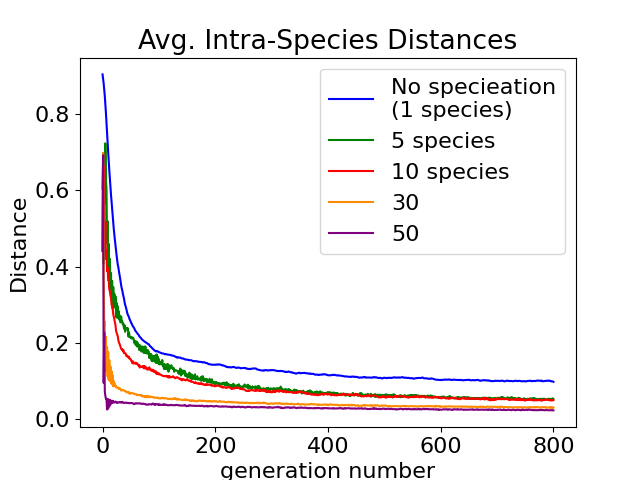
\includegraphics[width=15cm]{images/intraspecies_distance.png}
    \caption[Average intra-species distance over time]{Networks within a species become more similar over time.}
    \label{fig:avg_species_differences}
\end{figure}



\subsection{Speciation Effects}
\label{section:speciation}
In order to test the effects of speciation on population diversity and oscillator success rate, evolution was run without speciation, and with 10 and 30 as the target number of species. When speciation is disabled, the top 10\% of the entire population is passed on to the next generation unmodified and the bottom 10\% of the entire population is deleted. Then mutation is performed on the entire population to populate the remainder of the subsequent generation (crossover was not performed for these experiments). Each network must compete against every other network in the population. To account for fluctuations in population size when speciation is enabled, diversity was measured as the number of unique networks over the total number of networks in the population. A network was considered unique if differed by one or more reactions from all other networks. Reactions are considered different if they differ in product or reactant. Rate constants are not considered in these comparisons. Significance levels were calculated using two-tailed t-tests. 


In trials where no speciation was allowed, the average portion of unique networks was 0.294 $\pm$ 0.035 across 800 generations. This is significantly (p \textless xxx) less than the portion of unique networks in evolution trials with a target number of species of 10, 0.344 $\pm$ 0.037 (figure \ref{fig:num_unique_species}).

\begin{figure}
\centering
    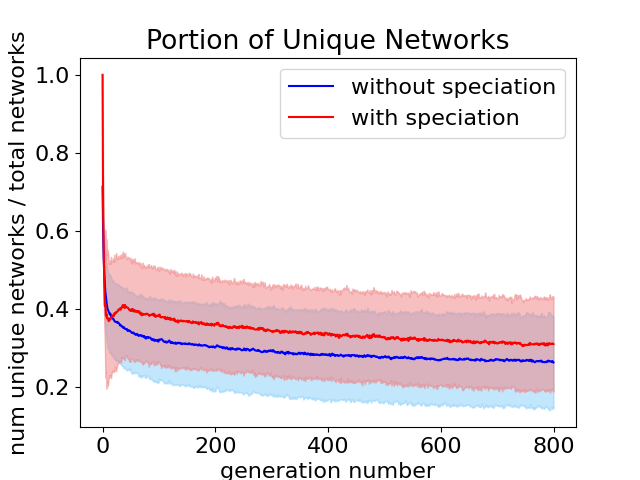
\includegraphics[width=15cm]{images/num_unique_networks.png}
    \caption[Unique networks with and without speciation]{The average portion of unique networks over 800 generations with speciation (red), 0.344 $\pm$ 0.037, and without (blue), 0.296 $\pm$ 0.034. Shading is the 95\% confidence interval.}
    \label{fig:num_unique_species}
\end{figure}

One purpose of speciation was to prevent the most fit network from overtaking the population over time. When a single network dominates the population, there are not enough unique networks to adequately explore the solution space and the evolution algorithm converges on a solution prematurely. To account for fluctuating population sizes when speciation is allowed, the number of copies of the best network divided by the total number of networks was measured at each generation with speciation (with a target species number of 10) and without speciation.  When speciated was enabled, the portion of the population occupied by copies of the most fit network
remained constant with an average portion of best networks of 0.071 $\pm$ 0.008. Without speciation, the portion of best networks rose gradually over time with an average portion of 0.402 $\pm$ 0.079 (figure \ref{fig:portion_best_network}). This shows that speciation effectively prevents a single network from dominating the population (p \textless 0.0001).

\begin{figure}
	\centering
    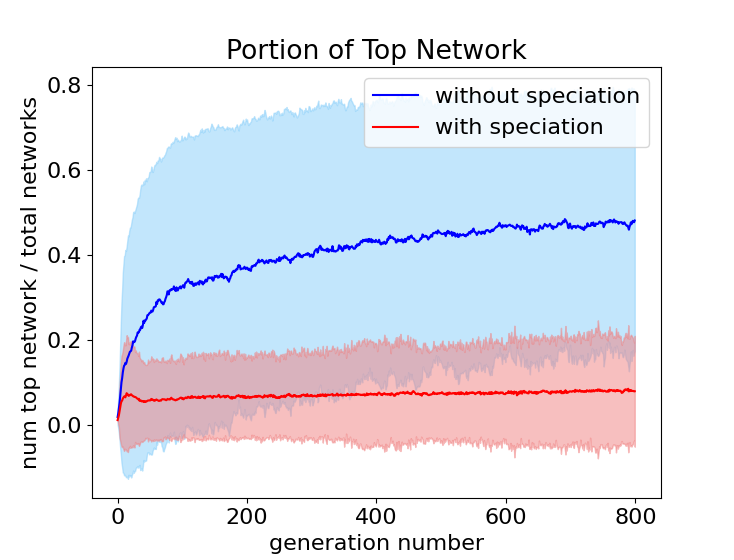
\includegraphics[width=18cm]{images/portion_best_network.png}
    \caption[Portion of top network over time, with and without speciation]{The average portion of best networks over 800 generations with speciation (red), 0.071 $\pm$ 0.008, and without (blue), 0.402 $\pm$ 0.079. Shading is the 95\% confidence interval.}
    \label{fig:portion_best_network}
\end{figure}


Next, the effects of speciation on evolution success rate was evaluated comparing no speciation to speciation with a target species number of 10, 30, and 50 (figure \ref{fig:species_success_rate}. Again, crossover was omitted from these studies. For each speciation level, a batch of 700 trials of evolution were run and the number of oscillators resulting from each batch. Significance levels were calculated using a binomial test. 

With a target species of 10 (the default condition), evolution trials resulted in sustained oscillators at a rate of 0.22 (154/700). Without speciation, the success was significantly reduced (p \textless 0.0001), with oscillators occurring at a rate of 0.12 (83/700). To more thoroughly evaluate the benefits of speciation, two more evolution batches (with 700 trials each) of evolution were run with target species of 30 and 50. The batch with a target of 30 species also had a success rate of 0.22 (153/700). Increasing the target number of species to 50 significantly (p=0.002) worsened results with a success rate of 0.16 (110/700). This success is still a significant improvement over evolution without speciation (p \textless 0.0001).

Speciation increases the success rate of evolution by sheltering innovations and maintaining population diversity. However, with too many species, there are not enough individuals in any given species to adequate explore the space and the success rate is reduced.

 
\begin{figure}
	\centering
    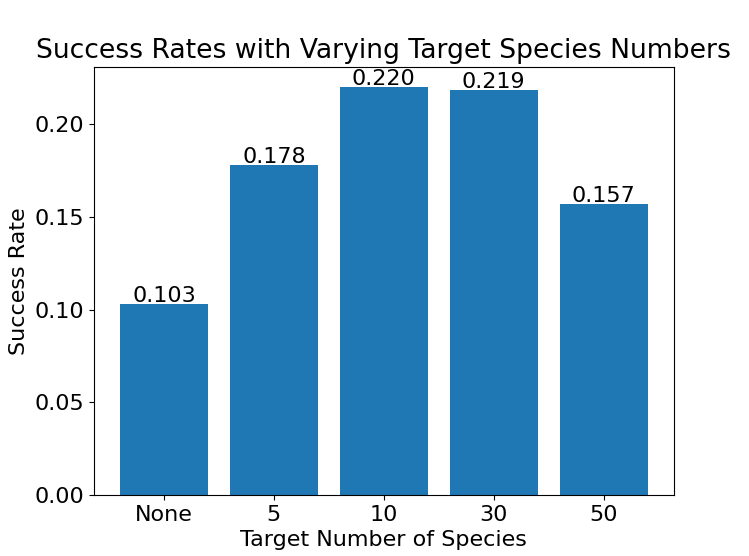
\includegraphics[width=15cm]{images/species_success_rate.png}
    \caption[Evolutionary success rate with varying target species numbers]{Evolution success rate of 700 trials with no speciation and with a target species of 5, 10, 30, and 50.}
    \label{fig:species_success_rate}
\end{figure}

\subsection{Crossover}
To assess the effects of crossover on evolutionary success, batches of 700 evolution trials without crossover and with several type of crossover were compared. None of the crossover batches tested here had better evolutionary success than the batch without crossover. 

First, the crossover technique described previously was compared to a batch with no crossover. Both batches had a target species of 10 and all other parameters in common. The batch with without crossover had 0\% chance of crossover and 100\% chance of mutation.  22\% (154/700) of trials in this batch resulted in oscillators The batch with crossover used the crossover procedure described in the Methods section. The probability of crossover was 0.75 and the probability of mutation was 0.75. All networks were either crossed over or mutated ($p_{crossover} + p_{mutation} - p_{crossover} \cap p_{mutation} = 1$). This meant that networks had a 50\% chance of being crossed over and then mutated ($p_{crossover} \cap p_{mutation} = p_{crossover} + p_{mutation} -1$). With these settings, evolution trials with crossover resulted oscillators at a rate of 17\% (119/700) of the time. This was significantly lower than the success rate without crossover (p = 0.001181).

It's possible that allowing some networks to undergo both crossover and mutation was too much change in a single step and was disrupting any progress towards a solution. In the next batch, networks were only allowed to undergo crossover or mutation (50\% of each), but never both. In this case, 13.7\% (96/700) trials resulted in oscillators, significantly less than both the batch without crossover and the batch with the original crossover method.

In a second attempt to address the problem of too much change, the probably of crossover was reduced from 0.75 to 0.25. For this batch, 20.6\% of trials resulted in oscillators. This is significantly better than the batch with a 0.75 probability of crossover (p=0.014), but not significantly different than the batch with no crossover. 

With the original crossover method described in \ref{section: crossover}, when two networks have the exact same fitness, one is randomly chosen as the more fit network. It is highly improbable that two networks would have exactly the same fitness, but this prompted the thought that there may be some benefit to more leniently combining two networks with similar fitness scores. For the next batch, networks with a fitness score within 5\% of one another underwent a slightly different crossover method. Like the original crossover method, all reactions that were present in both parent networks were passed to the offspring, with the rate constant chosen randomly from one parent or the other. Reactions that were not shared between the two networks were passed down with a 0.5 probability. As with the original crossover method, reactions that were inactive had a 0.25 probability of reactivation. The success of this batch (16.1\%, 111/700) was no different than the success of the original crossover batch and both were worse than the batch without crossover (p \textless 0.0001).

\begin{figure}
	\centering
    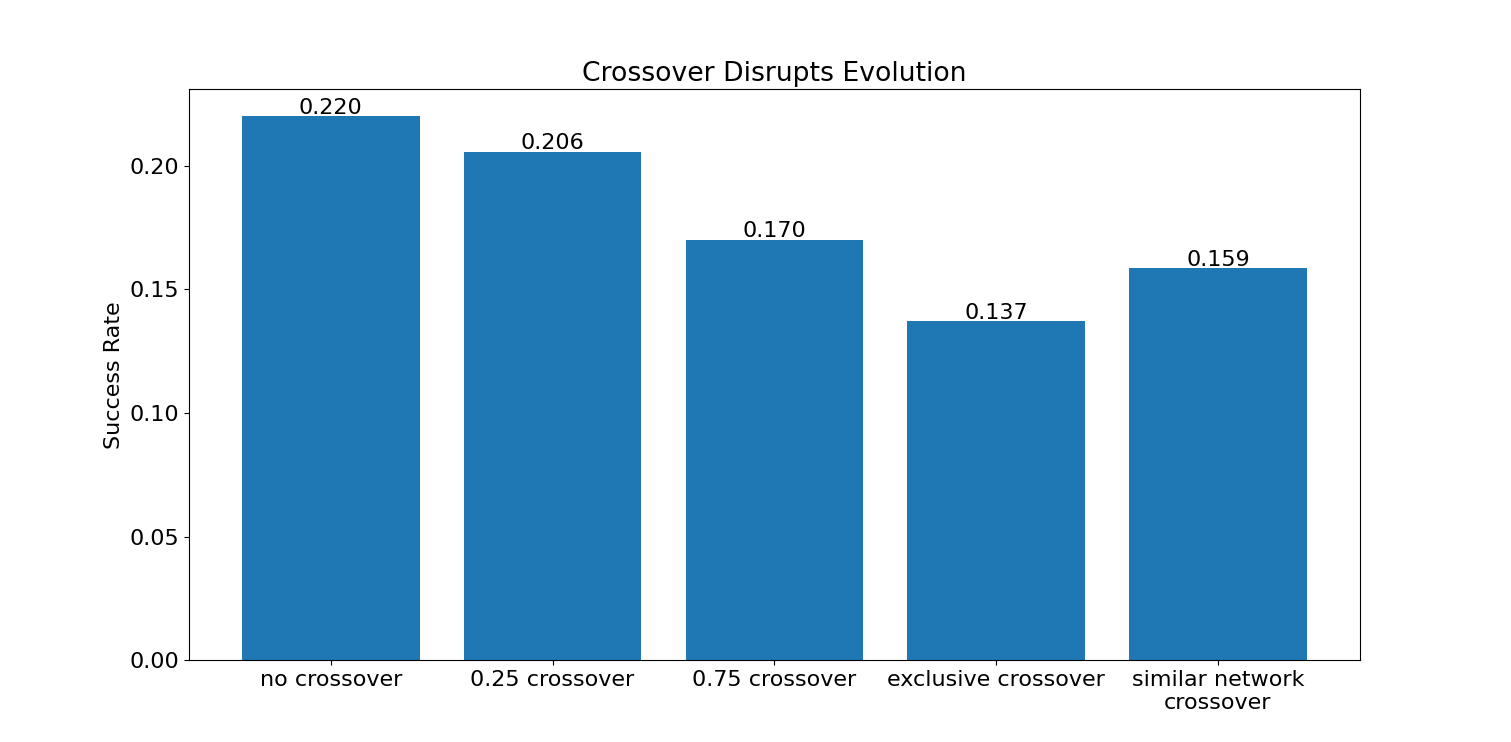
\includegraphics[width=18cm]{images/crossover_success.png}
    \caption[Evolutionary success rate with different crossover strategies]{Evolution success rate of 700 trials with no crossover, 0.25 and 0.75 probability of crossover, 50-50 exclusive chance of crossover or mutation, and 0.75 probability of crossover with more lenient crossover method for networks with similar fitness.}
    \label{fig:crossover_success}
\end{figure}


\subsection{Elitist Selection}
\label{section:elites}
Populating each generations begins with elitist selection. For each species, 10\% of its allocated offspring are unmodified copies of the best networks from the previous generation. In cases where a species is only allocated a single offspring, a mutation is performed on the best network in the species. If the mutation improves the network, the network is passed on to the next generation with the mutation. If the mutation does not improve the network, the unmodified network is passed on to the next generation.

To explore the influence of elitist selection, batches of 700 trials of evolution were run with and without elitism. For batches with elitism, levels of 10, 25, and 50\% were tested\footnote{This is the percentage of the \textit{next} generation that is composed of unmodified, higher fitness models. For example, if a species has 20 members but is only allowed 10 offspring with an elitism rate of 10\%, then the single best network of the 20 will be passed down to the next generation unmodified.}. Eliminating elitism resulted in drastically reduced success rates, with only 1\% (7/700) trials resulting in oscillators. However, in batches with elitism, the percentage of high fitness models copied to the next generation did not result in significantly different success rates. Batches with 10, 25, and 50\% elitism had success rates of 0.220 (154/700), 0.224 (157/700), and 0.197 (138/700) respectively (figure \ref{fig:elitism_success}). It is likely that evolution is driven primarily by the top few individuals. When elitism is removed, these top individuals are not preserved and evolution mostly fails. However keeping more individuals in addition to these top performers does not improve success rates.

\begin{figure}
	\centering
    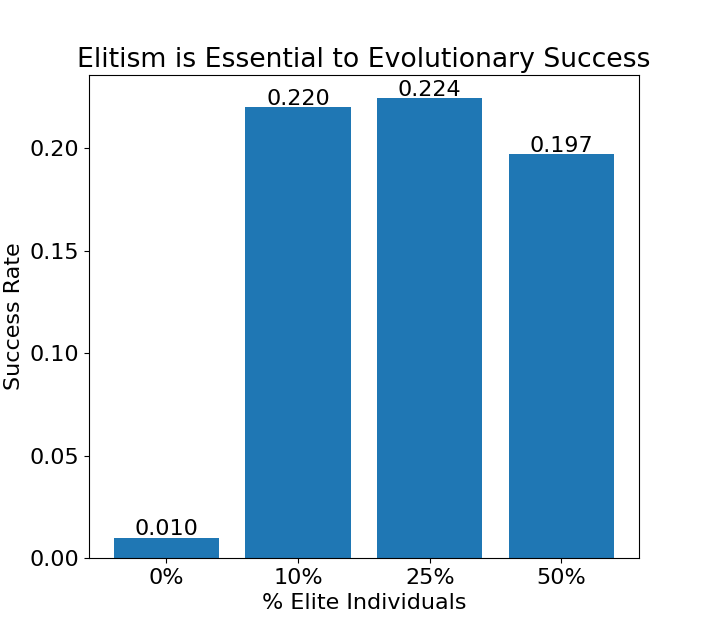
\includegraphics[width=15cm]{images/elitism_success.png}
    \caption[Evolutionary success rate with different levels of elitist selection]{Evolution success rate of 700 trials with no speciation and with a target species of 10, 30, and 50.}
    \label{fig:elitism_success}
\end{figure}


\subsection{Tournament Selection}
After the elite networks were copied to the next generation, the remaining offspring were produced by randomly selecting networks (including the elites, excluding the bottom 10\%) to mutate or crossover. As demonstrated in section \ref{section:elites}, elitism is crucial to the algorithms success. But could a different selection strategy for the non-elite offpsring improve success rate? To test this, tournament selection, with and without speciation, was used to select the non-elite offspring.

Tournament selection involves running several comparisons of a few individuals chosen at random from the population \cite{tournamentselect,  Miller1995}. The best of the subset is chosen for crossover or mutation. It is efficient to code and scales well population size and objective function. In this case, two individuals from the same species were randomly chosen (with replacement) and the individual with the better fitness score was allowed to mutate or crossover and continue to the next generation.

Tournament selection trials with a target species number of 10 and without speciation were compared to trials where non-elite networks were randomly selected. The trial with tournament selection and no speciation performed worst, with only 7.5\% of trials resulting in an oscillator (105/1400). With random selection, 11.1\% of trials resulting in oscillators (155/1400). This difference is statistically significant with p \textless 0.0001. This result was unexpected, as it would seem that biasing selection towards more fit networks with tournament selection should improve the results. However, it is possible that random selection helped maintain diversity by including less fit networks that ultimately developed into good solutions.

When considering tournament selection with speciation, results improved, with 21.1\% (148/700) of trials resulting in an oscillator. However, this result in not significantly different than random selection with speciation, which resulted in oscillators in 22.0\% of trials (154/700). This bolsters the conclusion that speciation drives evolutionary success more than any other factors explored here.

\begin{figure}
	\centering
    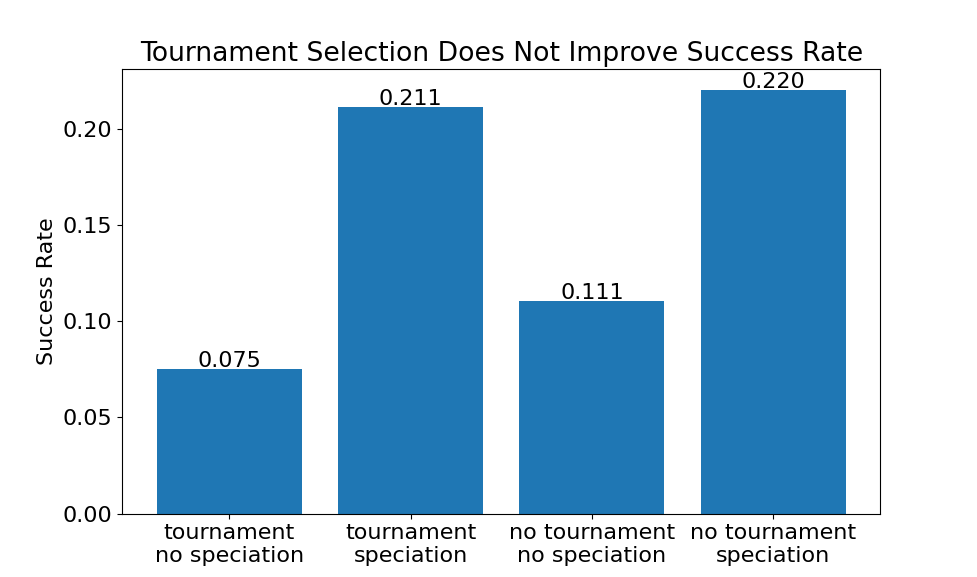
\includegraphics[width=15cm]{images/tournament_speciation.png}
    \caption[Evolutionary success rates with tournament selection and speciation]{Evolution success rate with and without tournament selection and with and without speciation. Speciation influences success rate far more than tournament selection (n=1400 for each no speciation batch, n=700 for speciation batches).}
    \label{fig:elitism_success}
\end{figure}

\subsection{Increased Population size}
Unlike other hyperparmaters discussed here, increasing the population size has a direct effect on computation time. The bulk of the algorithm consists of numerically solving the ODEs for each network. However, increasing the population size increases the number of individuals exploring the solution landscape and thus increases the chances of finding a good solution. 

When the population size was doubled, from 100 individuals to 200 individuals, evolutionary success significantly improved from 22\% to 26\% (p = 0.012), with 182 of 700 trials producing an oscillator. However, this computation took roughly twice as long. The batch with 100 individuals resulted in 154 oscillators (out of 700 trials). Running this batch twice would result in ~300 oscillators and take roughly the same amount of time as a 200 individual population that produces ~180 oscillators.

Next, a batch with a population of 200 and a target of 20 species was run. For a population of 100, a target species of 10 was shown to result in the highest success rate, so this experiment sought to test if the optimal target number of species scaled with population size. This appeared to be the case as 38.5\% (77/200) trials in this batch resulted in oscillators, a significant improvement over both 200 individuals with 10 species and 100 individuals with 10 species. 

\subsection{More Generations}
Like population size, the number of generations directly effects computation time. However, increasing the number of generations allows more time for the algorithm to discover and optimize solutions and increase evolutionary success. 

The maximum number of generations was doubled, from 800 to 1600, and evolution was run with default parameters: no crossover, 100 individuals, target species of 10. Trials in this batch resulted in oscillators 37\% (74/200) of the time. Fit fitness of the top network in each generation was measured and the average fitness of the top networks across 200 trials is shown in figure \ref{fig:1600_top_fitness}. After 1600 generations, the average top fitness continues to rise suggesting that the success rate may further increase with more generations. When the number of generations was doubled again, from 1600 to 3200, the success rate was 50\% (100/200).
 

\begin{figure}
\centering
    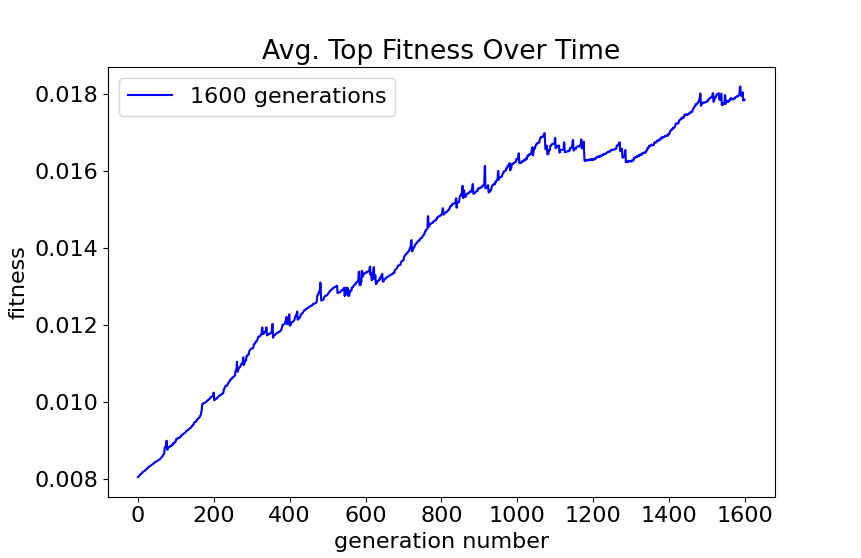
\includegraphics[width=15cm]{images/1600_top_fitness.png}
    \caption[Average top fitness over 1600 generations]{Average fitness of the best network of each generation over 200 trials. Small spikes can likely be attributed to writing out networks with high fitness and discontinuing evolution trials.}
    \label{fig:1600_top_fitness}
\end{figure}

\subsection{fitness function with rate constants}


\subsection{Maybe: optimal parameters}

\subsection{Matching Time Series Data}
Beyond generating oscillators, the NetEvolve software is intended to implement an evolutionary algorithm for more broad systems biology problems. One application could be evolving reaction networks that match time series data. To test if NetEvolve could generate networks to match time series data, a simple, 3 chemical, 5 reaction synthetic network was constructed and its time series data collected (figure \ref{fig:groundtruth}). Then the NetEvolve software was given the time series data as an objective. 

\begin{figure}
\centering
    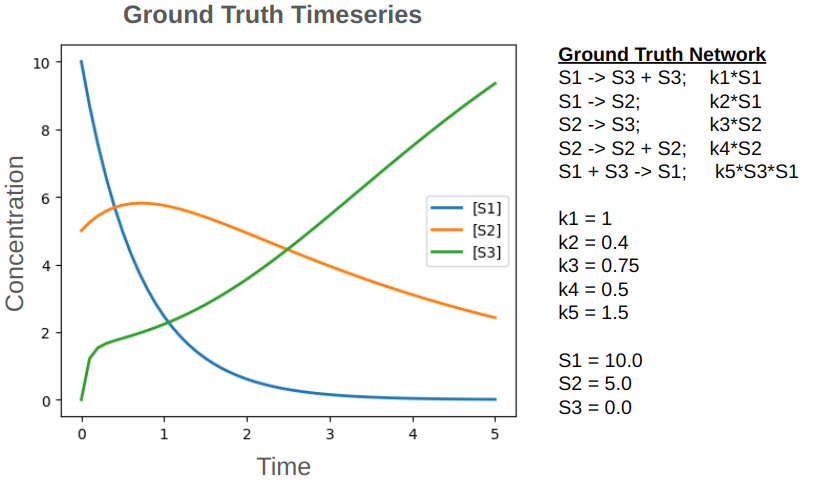
\includegraphics[width=18cm]{images/groundtruth.png}
    \caption[A ground truth synthetic network and its time series]{A synthetic network and its time series data.}
    \label{fig:groundtruth}
\end{figure}

Four hundred trials of evolution were run, each with 1600 generations in an effort to match the ground truth time series data. The 12 best matching evolved time series are shown in figure \ref{fig:12_timeseries}. The time series data of the 12 best evolved networks all closely match the dynamics in the ground truth network. The best matching time series (top row left of figure \ref{fig:12_timeseries}) is shown overlaid with the ground truth time series in figure \ref{fig:truth_vs_evolved}. The solid lines are data from the ground truth network and the dashed lines are from the evolved network.

\begin{figure}
\centering
    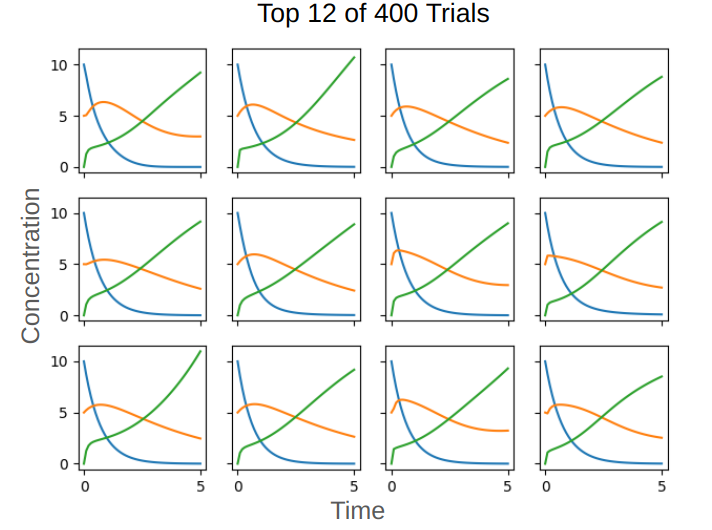
\includegraphics[width=15cm]{images/12_timeseries.png}
    \caption[The 12 trials that most closely matched the time series data]{The 12 trials that most closely matched the time series data.}
    \label{fig:12_timeseries}
\end{figure}

\begin{figure}
\centering
    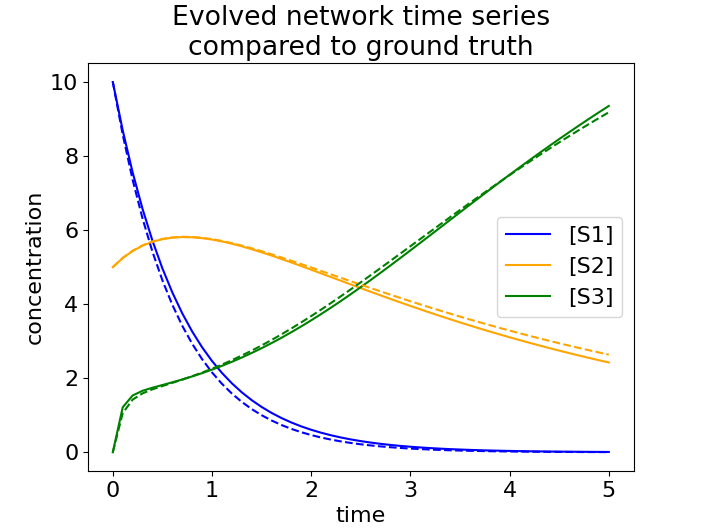
\includegraphics[width=15cm]{images/ground_truth_vs_evolved.png}
    \caption[Time series of the ground truth network compared to the best evolved network]{Time series of the ground truth network (solid lines) compared to the best evolved network (dashed lines).}
    \label{fig:truth_vs_evolved}
\end{figure}

Interestingly, the evolved network that most closely matched the ground truth time series data only had one reaction in common with the original network (figure \ref{fig:evolved_network_structure}). Of the 12 best evolved networks the third best network had the most reactions, 3 of 5, in common with the original network. The last reaction, S1 + S3 $\to$ S1, occurred in 10 of the 12 best networks. The next most common was the reaction S2 $\to$ S3, which occurred in 7 of the 12 best networks. All networks that had the reaction S2 $\to$ S3 also had the reaction S1 + S3 $\to$ S1.

\begin{figure}
\centering
    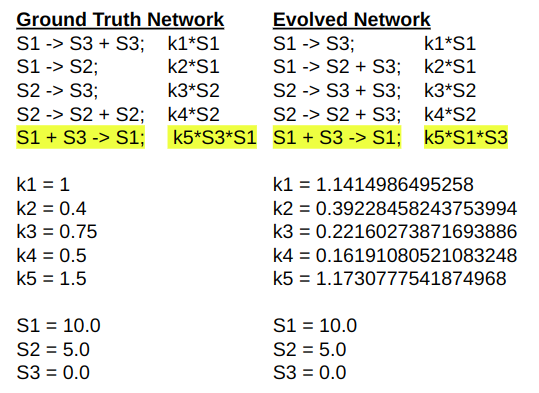
\includegraphics[width=15cm]{images/antimony_truth_evolved.png}
    \caption[The ground truth network compared to the best evolved network]{The ground truth network compared to the best evolved network}
    \label{fig:evolved_network_structure}
\end{figure}

\section{Discussion}
Speciation was shown to signficantly benefit evolutionary success by protection innovations and maintaining evolutionary diversity throughout the process. Fine tuning is necessary to achieve the maximum benefit of speciation. The target number of species must be chosen with consideration of the population size. Additionally, $\delta$ and $\delta$ step sizes may require adjustment for different population sizes, target number of species, and different objectives. 

Elitism is also essential to evolution as it preserves the best individuals of each generation. It pairs well with speciation as it allows the best individuals not just from the whole population but from the each species to be passed on to the next generation. Interestingly, the evolutionary success did not seem to vary with different levels of elitism suggesting that evolutionary progress is driven primarily by the top individuals of each species and that including additional elite networks does not improve success. This seems to be confirmed by the observation that alternative selection strategies for non-elite individuals did not affect evolutionary performance.

Although crossover has shown success in other topological evolution problems \cite{stanley_evolving_2002, dinh_effective_2015}, this was not the case with mass-action networks. Both artificial neural networks (ANNs) and genetic regulatory networks (GRNs) (domains where crossover has been shown effective) have more edges that can more easily be separated from their weights. In both cases, edges simply connect two nodes together. For ANNs, all edges activate the output node and have a weight which increases or decreases the signal strength. GRNs are similar but edges can also be inhibitory. The weights of the edges are not influence by the nodes the edge is connected to. On the other hand, in this work, reactions are analogous to edges and can connect two to four nodes (chemical species). The rate constants are analogous to weights. But unlike weights, the extent to which one node activates another (or the speed at which a reactant becomes a product) is also influenced by the reactant's concentration. That is to say, in the case of mass-action chemical reaction networks, it is far more difficult to isolate subsets of a network and maintain their function. When crossover occurs, it tends to disrupt the finely tuned developing solutions by changing several rate constants simultaneously. This could explain why crossover reduces success in this application despite its utility in other domains. 

Although this algorithm is faster than previous iterations, it still computationally expensive. A single trial of 800 generations and 100 individuals take approximately 90 seconds on average. The vast majority of this time is consumed by numerically solving the ODEs. The software uses a custom function to compute the rate of change of each concentration, but the solver is from julia's DifferentialEquations and Sundials libraries, both highly optimized for performance. Additionally, the software uses strict typing, pre-allocation wherever possible, and hash maps to further improve performance. Although the current implementation of NetEvolve does not make use of parallelization within a single trial, in practice multiple trials can be dispatch to different CPUs using a bash script or job array. Improving success rate in future iterations would likely prove more beneficial than slightly increasing computational performance.


Using an adaptive speciation threshold, $\delta$, did not directly influence evolutionary success, but it maintained the target number of species which did influence success. Without an adaptive $\delta$, the user would have to manually tune $\delta$ through trial and error to achieve the target number of species. Given the utility of this adaptive feature, it may be useful to implement a similar strategy for other evolutionary hyperparameters. For example, the probability of changing the topology (adding or deleting reactions) versus changing rate constants remains the same throughout the evolutionary process. Early on, it may be useful to change topology more frequently in an effort to find a decent solution. However, later in the process, when hopefully a promising solution has been found, it is more useful to modify rate constants in an effort to optimize the solution. Changing topology may be wasted effort and may divert resources that may be better spent optimizing an existing solution. In future iterations of NetEvolve, it may be useful to change the balance of topological versus rate constant mutation over time or as fitness reaches a pre-specified threshold.

Similarly, as evolution progresses and homes in a promising solution, smaller rate constant changes may be necessary to explore a small area in the solution space in more detail. The amount by which rate constants are changed could be adaptively reduced over time, either based on fitness or generation number. 

Another means of more thoroughly exploring a promising solution space as evolution progresses could be altering the metric used to determine the ``distance" between two networks, and thus their species. In the current iteration of NetEvolve, the distance between two networks is entirely determined by the amount of reactions that the two networks do not share with no consideration to the rate constants for shared reactions. Networks with the same topology are considered identical even if rate constants for their different reactions vary by orders of magnitude. Including the differences in rate constants when considering distance could improve evolution by encouraging more thorough explorations of viable solution spaces towards the end of the process. As networks become more similar topologically as evolution progresses, including rate constants in the distance metric would encourage speciation based on on how much parameters differ. This would direct more resources towards optimizing a decent solution as opposed to continuing to explore the broader solution space.

One flaw of the existing iteration of NetEvolve is the tendency to add extraneous reactions. It appears that more often than not, deleting a reaction reduces fitness whereas adding a reaction may slightly improve fitness. Although there was equal probability of adding and deleting reactions, networks at the end of evolution tended to be much larger (~15 reactions) than at the start (5) reactions. In some cases, this may not be of concern. For example, if the goal is simply to create a population of oscillators, it may not matter that some of them are overly complicated. However, if attempting to gather simple networks to fit time series data, the tendency to over complicate networks could be detrimental. Overfitting by over complicating models (for example, by including too many predictors) is a well-known problem in machine learning. Often, the solution is to penalize models that use too many features. A similar technique could be implemented here, penalizing candidate networks for each additional reaction. 

Additionally, the algorithm has demonstrated its ability to produced oscillators, but its ability to match other network behaviors is untested. It successfully generated a network to match simple time series data, but did not manage to recover the network that produced the data. More testing and algorithm development could improve NetEvolve's performance in tasks beyond generating oscillators. 

\section{Conclusion}
Yay I did it.
\\


	
\chapter{Logistic Considerations for NetEvolve}

\section{Introduction}
The purpose of this chapter is to briefly describe the logistics of acquiring, using, and customizing the NetEvolve software. Several settings and some applications not described in the previous chapter are mentioned here.

\section{Acquiring NetEvolve}
NetEvolve is currently available as a github repository. In the future, it will be registered as a julia package in the general registry to more easily download. The package requires the julia programming language, which can be downloaded with directions from the julia website, \url{https://julialang.org/downloads/ }.

In a terminal, clone the github repository, located at \url{https://github.com/ltatka/NetEvolve.git} and navigate to the nearly created NetEvolve directory.

\begin{tcolorbox}
\begin{verbatim}
git clone https://github.com/ltatka/NetEvolve.git
cd NetEvolve
\end{verbatim}
end{tcolorbox}

The julia programming language has a built in package manager allowing for the seamless download and activation of all dependencies in a virtual environment.
\begin{verbatim}
julia --project=. -e 'using Pkg; Pkg.instantiate()'
\end{verbatim}

The evolution algorithm can be run with the default settings via the following command:
\begin{verbatim}
julia --project=. run_evolution.jl
\end{verbatim}

The \verb+run_evolution+ command can be modified with several command line arguments to quickly customize the evolutionary algorithm. 

\begin{table}[]
\begin{tabular}{|l|l|}
\hline
\textbf{Flag}    & \textbf{Description}                                     \\ \hline
\verb+--ntrials+        & The number of evolutionary trials to run, 100 by default \\ \hline
\verb+--ngenerations+   & The number of generations for each trial, 800 by default \\ \hline
\verb+--populationsize+ & The number of individuals in each trial, 100 by default  \\ \hline
\verb+--pathtosettings+ & Path to a json file with custom settings                 \\ \hline
\verb+--outputpath+     & Path to directory where output networks will be written  \\ \hline
\verb+--seed+           & Random seed                                              \\ \hline
\caption[The ground truth network compared to the best evolved network]{The ground truth network compared to the best evolved network}
    \label{fig:evolved_network_structure}
\end{tabular}
\end{table}

- Intro
- how to get the software
- using the software
	- quickstart
	- Running with a bash script locally
	- submitting to cluster
- Uses:
	- evolve general behaviors such as oscillator
	- Match time series
	- Parameter fitting with no topology change
	
- THings you can customize


\begin{figure}
    \centering
    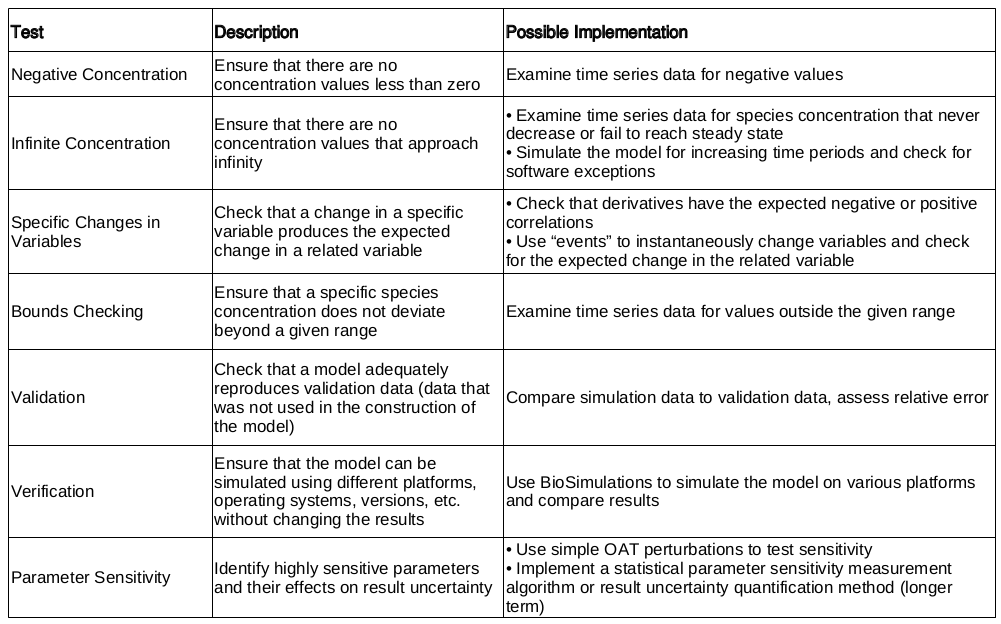
\includegraphics[width=19cm]{images/testSummary.png}
    \captionof{table}{Summary of proposed tests and possible implementations.}
    \label{table:sensitivity}
\end{figure}



% Bibliography
\bibliographystyle{plain}
\bibliography{researchbib}
\end{document}


